\chapter{Association analysis between symptomology and herpesvirus IgG antibody concentrations in ME/CFS and MS}
\label{chapter:2023-sym-and-herpesvirus}
\chaptermark{Association analysis between symptomology and\\herpesvirus IgG antibody concentrations in ME/CFS and MS}

%%%%%%%%%%%%%%%%%%%%%%%%%%%%%%%%%%%%%%%%%%%%%%%%%%%%%%%%%%%%%%%%%%%%%%%%
\noindent T.D. Domingues\footnote{\label{foot:contribution}Authors contributed equally to this work.}, \underline{J. Malato}\footref{foot:contribution}, A.D. Grabowska, J.-S. Lee, J. Ameijeiras-Alonso, P. Biecek, L. Graça, H. Mouriño, C. Scheibenbogen, F. Westermeier, L. Nacul, J.M. Cliff, E. Lacerda, and N. Sepúlveda. Association analysis between symptomology and herpesvirus IgG antibody concentrations in myalgic encephalomyelitis/chronic fatigue syndrome (ME/CFS) and multiple sclerosis. \textit{Heliyon}. 2023; 9(7):E18250. doi: \url{https://doi.org/10.1016/j.heliyon.2023.e18250}.


%%%%%%%%%%%%%%%%%%%%%%%%%%%%%%%%%%%%%%%%%%%%%%%%%%%%%%%%%%%%%%%%%%%%%%%%
\begin{abstract}
Myalgic encephalomyelitis/Chronic fatigue syndrome (ME/CFS) and multiple sclerosis (MS) are two complex and multifactorial diseases whose patients experience persistent fatigue, cognitive impairment, among other shared symptoms. The onset of these diseases has also been linked to acute herpesvirus infections or their reactivations. In this work, we re-analysed a previously-described dataset related to IgG antibody responses to 6 herpesviruses (CMV--cytomegalovirus; EBV--Epstein-Barr virus; HHV6--human herpesvirus-6; HSV1 and HSV2--herpes simplex virus-1 and -2, respectively; VZV--varicella-zoster virus) from the United Kingdom ME/CFS biobank. The primary goal was to report the underlying symptomology and its association with herpesvirus IgG antibodies using data from 4 disease-trigger-based subgroups of ME/CFS patients ($n = 222$) and patients with MS ($n = 46$). The secondary objective was to assess whether serological data could distinguish ME/CFS and its subgroup from MS using a SuperLearner (SL) algorithm. There was evidence for a significant negative association between temporary eyesight disturbance and CMV antibody concentrations and for a significant positive association between bladder problems and EBV antibody concentrations in the MS group. In the ME/CFS or its subgroups, the most significant antibody-symptom association was obtained for increasing HSV1 antibody concentration and brain fog, a finding in line with a negative impact of HSV1 exposure on cognitive outcomes in both healthy and disease conditions. There was also evidence for a higher number of significant antibody-symptom associations in the MS group than in the ME/CFS group. When we combined all the serological data in an SL algorithm, we could distinguish three ME/CFS subgroups (unknown disease trigger, non-infection trigger, and an infection disease trigger confirmed in the lab at the time of the event) from the MS group. However, we could not find the same for the remaining ME/CFS group (related to an unconfirmed infection disease). In conclusion, IgG antibody data explains more the symptomology of MS patients than the one of ME/CFS patients. Given the fluctuating nature of symptoms in ME/CFS patients, the clinical implication of these findings remains to be determined with a longitudinal study. This study is likely to ascertain the robustness of the associations during natural disease course.
\keywords{Enzyme-linked immunosorbent assay; Epstein-barr virus; Cytomegalovirus; Human herpesvirus-6; Varicella-zoster virus; Herpes simplex virus-1 and -2; SuperLearner; United Kingdom ME/CFS biobank}
\end{abstract}

%%%%%%%%%%%%%%%%%%%%%%%%%%%%%%%%%%%%%%%%%%%%%%%%%%%%%%%%%%%%%%%%%%%%%%%%
%%%%%%%%%%%%%%%%%%%%%%%%%%%%%%%%%%%%%%%%%%%%%%%%%%%%%%%%%%%%%%%%%%%%%%%%
%%%%%%%%%%%%%%%%%%%%%%%%%%%%%%%%%%%%%%%%%%%%%%%%%%%%%%%%%%%%%%%%%%%%%%%%
\section{Introduction}

Myalgic encephalomyelitis/Chronic fatigue syndrome (ME/CFS) is a widely neglected disease characterised by persistent fatigue, post-exertional malaise (PEM), unrefreshing sleep, among other symptoms related to multiple body systems \citep{rivera2019MyalgicEncephalomyelitis}. Despite the research efforts \citep{scheibenbogen2017EuropeanME}, there are no objective biomarkers for the diagnosis and prognosis of ME/CFS. The absence of this key clinical tool delays disease diagnosis and subsequent treatment \citep{nacul2021EuropeanNetwork}. It also slows down research progress due to lack of finding's reproducibility across studies \citep{nacul2019HowHave, malato2023ImpactMisdiagnosis}. Notwithstanding all these problems, there is a growing body of evidence for an autoimmune component for the origin and chronicity of the disease, especially in patients with an acute infection at their disease onset \citep{sotznyMyalgicEncephalomyelitisChronic2018, blomberg2018InfectionEliciteda, sepulveda2019MyalgicEncephalomyelitis, steiner2020AutoimmunityRelatedRisk}. The main candidate proteins for this deleterious autoimmune phenomenon are the adrenergic receptors \citep{loebel2016AntibodiesAdrenergic, bynke2020AutoantibodiesBetaadrenergic, freitag2021AutoantibodiesVasoregulative}. However, other human proteins, such as Anoctamin-2 and thyroid peroxidase, have also been suggested \citep{loebel2017SerologicalProfiling, sepulveda2021ImpactGenetic}.

The autoimmune hypothesis for the aetiology of ME/CFS directed research efforts towards the identification of key differences between ME/CFS and different autoimmune diseases, including multiple sclerosis (MS) \citep{ramosRegulatoryNaturalKiller2016, loebel2017SerologicalProfiling}. In this regard, patients with MS were deemed an important disease control group given that they experience chronic fatigue as a major manifestation of their disease. These patients and the ME/CFS ones also share some neurological symptoms, such as brain fog, memory loss, cognitive impairment, and photosensitivity/photophobia \citep{morrisMyalgicEncephalomyelitisChronic2013}. In addition, the root cause of both diseases has been linked to the infections by herpesviruses \citep{rasa2018ChronicViral, ariza2021MyalgicEncephalomyelitis, sedighi2022ComprehensiveInvestigations, rasa-dzelzkaleja2023PersistentViral, khalesi2023AssociationHuman}, such as Epstein-Barr virus (EBV) \citep{ruiz-pablos2021EpsteinBarrVirus, bjornevik2022LongitudinalAnalysis, soldan2023EpsteinBarr} and human herpesvirus-6 (HHV6) \citep{engdahl2019IncreasedSerological, lee2021SalivaryDNA, lundstrom2022HumanHerpesvirus, kasimir2022TissueSpecific}. Finally, it was recently hypothesised that ME/CFS and MS share reduced craniospinal compliance and dilated pressured bridging cortical veins \citep{bateman2024ChronicFatigue}.

The similarity between these two diseases also prompted the creation of the United Kingdom ME/CFS biobank (UKMEB), a large sample resource for the research community, where patients with MS were included as a disease control group \citep{lacerda2017UKME, lacerda2018UKME}. Until now, most of the UKMEB-based studies compared ME/CFS patients to healthy controls \citep{rodrigues2019HERVKHERVW, almenar-perez2020AssessingDiagnostic, blauensteiner2021AlteredEndothelial, bertinat2022DecreasedNO, vogl2022SystemicAntibody, gonzalez-cebrian2022DiagnosisMyalgic} with a few exceptions where the MS group was also included in the analysis \citep{jain2017PrevalenceRisk, lacerdaLogisticRegressionAnalysis2019, melvin2019CirculatingLevels, cliff2019CellularImmune}. For example, one study reported significant differences in the frequency of several immune-cell populations between MS and ME/CFS patients \citep{cliff2019CellularImmune}; however, some of these differences were not found when comparing these groups to healthy controls. The same study showed that MS patients had a significantly higher seroprevalence to EBV-derived nuclear antigen-1 (EBNA1) antigen when comparing to both healthy controls and ME/CFS patients divided according to their disease severity. Another study reported evidence for similar average concentration of the stress-related growth/differentiation factor 15 peptide between MS and ME/CFS group \citep{melvin2019CirculatingLevels}. Therefore, it is important to increase current knowledge about the pathological differences between ME/CFS and MS using data from the UKMEB.

In a previous study, we divided the cohort of ME/CFS patients from the UKMEB into 4 subgroups according to their putative disease triggers and compared them to healthy controls in terms of IgG antibody responses to 6 herpesviruses \citep{domingues2021HerpesvirusesSerologya}. We found reductions in antibody concentrations to EBV in the ME/CFS subgroup without a putative infection trigger and to CMV in the ME/CFS subgroup with a confirmed infection at disease onset. In the present study, we analysed symptoms data from the UKMEB using the MS cohort as the control group and assessed the respective association with the same herpesvirus IgG antibody data mentioned above. We also integrated the IgG antibody data in a SuperLearner (SL) algorithm with the objective of assessing the classification power to distinguish each ME/CFS subgroup from the MS one. Overall, our analyses aimed at providing new data on what differentiates ME/CFS and its subgroups from MS. Given that there are more published studies related to the role of herpesviruses on MS than on ME/CFS, most of the findings reported here are not particularly novel (e.g., high EBV IgG antibody concentrations) for this disease.

%%%%%%%%%%%%%%%%%%%%%%%%%%%%%%%%%%%%%%%%%%%%%%%%%%%%%%%%%%%%%%%%%%%%%%%%
%%%%%%%%%%%%%%%%%%%%%%%%%%%%%%%%%%%%%%%%%%%%%%%%%%%%%%%%%%%%%%%%%%%%%%%%
%%%%%%%%%%%%%%%%%%%%%%%%%%%%%%%%%%%%%%%%%%%%%%%%%%%%%%%%%%%%%%%%%%%%%%%%
\section{Materials and methods}

%%%%%%%%%%%%%%%%%%%%%%%%%%%%%%%%%%%%%%%%%%%%%%%%%%%%%%%%%%%%%%%%%%%%%%%%
\subsection{Study participants}

The study participants were 222 adult patients with ME/CFS and 46 adult patients with MS whose serological data were available from the UKMEB. As in our previous study \citep{domingues2021HerpesvirusesSerologya}, we divided patients with ME/CFS into the following four subgroups according to the disease trigger: S0--an unknown trigger ($n = 42$); S1--a non-infectious trigger ($n = 42$); S2--an infection that was not evaluated by a lab test at the time of the event ($n = 92$); and S3--an infection that was confirmed by a lab test at the time of the event ($n = 46$). The diagnosis of these patients complied with either the 1994 US Center for Disease Control and Prevention criteria (CDC-1994) \citep{fukuda1994ChronicFatigue} or the 2003 Canadian Consensus Criteria (CCC-2003) \citep{carruthers2003MyalgicEncephalomyelitis}. All putative study participants were excluded if they had (i) taken antiviral medication or drugs known to alter immune function in the preceding 3 months; (ii) had any vaccinations in the preceding 3 months; (iii) had a history of acute and chronic infectious diseases, such as hepatitis B and C, tuberculosis, HIV (but not herpes virus or other retrovirus infection); (iv) another chronic disease such as cancer, coronary heart disease, or uncontrolled diabetes; (v) a severe mood disorder; (vi) been pregnant or breastfeeding in the preceding 12 months; or (vii) were morbidly obese (BMI $\geq40$). Further information on the UKMEB can be found elsewhere \citep{lacerda2017UKME, lacerda2018UKME}. The severity of ME/CFS patients was divided into mild/moderate and severely affected (home or bed bound). MS patients had a previous diagnosis made by neurologists from the UK National Health System. No assessment of disease severity was made for these patients.

%%%%%%%%%%%%%%%%%%%%%%%%%%%%%%%%%%%%%%%%%%%%%%%%%%%%%%%%%%%%%%%%%%%%%%%%
\subsection{Symptomology assessment}

At the recruitment, all the study participants were asked to report their disease duration and disease course. They also answered a symptom's assessment questionnaire
%\textcolor{red}{(supplied as Supplementary Material, question \#13)} 
on the presence or absence of 58 different symptoms in the previous 7 days (Supplementary Table~\ref{appendix:taba1-sym-bin-description}). The symptoms were related to the following domains: autonomic ($n = 10$); immunological ($n = 9$); neuroendocrine ($n = 6$); neurocognitive (n = 19); pain ($n = 6$); post-exertional malaise ($n = 6$); and sleep function ($n = 2$). The frequency of each symptom per study group can be found in Supplementary Table~\ref{appendix:taba2-percentage-sym-bin}.
% Supplementary Table 1
% Supplementary Table~\ref{appendix:taba1-sym-bin-description}

% Supplementary Table 2
% Supplementary Table~\ref{appendix:taba2-percentage-sym-bin}

%%%%%%%%%%%%%%%%%%%%%%%%%%%%%%%%%%%%%%%%%%%%%%%%%%%%%%%%%%%%%%%%%%%%%%%%
\subsection{Herpesvirus IgG antibodies}

As mentioned in the Introduction, we re-analysed the same herpesvirus IgG antibody concentration dataset, as described in the original and follow-up study \citep{cliff2019CellularImmune, domingues2021HerpesvirusesSerologya}. Briefly, antibody quantification of each participant was performed at recruitment using different commercial ELISAs. Data referred to plasma concentrations (in arbitrary units per millilitre, U/ml) of IgG antibodies against human cytomegalovirus (CMV), EBV (EBNA1 and EBV-derived Viral Capsid Antigen, EBV-VCA), HHV6, herpes simplex virus-1 (HSV1), herpes simplex virus-2 (HSV2), and varicella-zoster virus (VZV). In the manufacturer's protocols, the suggested cutoff values for seropositivity were 12 U/ml for HSV1, HSV 2, VZV, CMV and EBV, and 12.5 U/ml for HHV6. The maximum of plasma concentrations per antibody was the following: CMV--304 U/ml; EBV-EBNA1--200 U/ml; EBV-VCA--468 U/ml; HHV6--419 U/ml; HSV1--257 U/ml; HSV2--367 U/ml; VZV--301 U/ml. Given that these maximum values translated into a narrow fold change in $\log_{10}$ scale beyond the seropositivity cut-off values, we chose to present some of the results using $\log_{2}$ scale.

%%%%%%%%%%%%%%%%%%%%%%%%%%%%%%%%%%%%%%%%%%%%%%%%%%%%%%%%%%%%%%%%%%%%%%%%
\subsection{Statistical analysis}

Basic quantitative characteristics (e.g., age and disease duration) were summarised by means, median, min, max, and standard deviation. Absolute frequencies and percentages were used for summarising basic categorical variables (e.g., gender and disease course). To compare different study groups in terms of these data, we used the non-parametric Kruskal-Wallis test and the Pearson's $\chi^2$ test for quantitative and categorical variables, respectively. We used a significance level of 5\% in these tests.

Symptomology data from the UKMEB were here analysed for the first time. In this analysis, we removed 9 symptoms, because the frequency of missing data was higher than 25\% in each disease group or overall. For each symptom, we calculated an age-adjusted odds ratio (OR) and the respective confidence interval using a logistic regression model where age was included as a confounding factor and MS was used as the reference group. The level of each confidence interval was adjusted by the Bonferroni correction to ensure a global confidence level of at least 95\%. This correction was used due to its tendency to be more conservative towards the null hypothesis (i.e., absence of association/homogeneity between groups).

With respect to serological data, we first estimated seroprevalences in each study group by the proportion of individuals above the cutoff points recommended by the respective ELISA protocol. We calculated the respective 95\% confidence interval using the Pearson-Clopper exact method. We performed the Pearson's $\chi^2$ test to assess the homogeneity of seroprevalences to a given herpesvirus. For the respective quantitative data, we reported the median and the interquartile range (IQR) in each study group and herpesvirus antibody. To compare the median antibody concentrations across all study groups, we performed the non-parametric Kruskal-Wallis tests using a significance level of 5\%.

Similarly to our previous study \citep{domingues2021HerpesvirusesSerologya}, we computed the Receiver Operating Characteristic (ROC) curve for each serological data, using all possible cut-off values to discriminate cases (ME/CFS subgroups) from controls (MS patients). We then estimated the respective areas under these curves (AUC) and computed their 95\% confidence interval. For this estimation, we checked whether antibody concentrations of cases were either higher or lower than controls and chose the direction that provided the maximum AUC. In this analysis, there was evidence for a random classification if the confidence intervals for AUC included the value 0.5. We finally computed the optimal cut-point for each of these ROC curves by maximising the significance of association provided by the Pearson's $\chi^2$ test. We finally adjusted the p-values associated with a given serological variable for multiple testing using the Benjamini-Hochberg procedure \citep{benjaminiControllingFalseDiscovery1995}. This adjustment ensured a global false discovery rate (FDR) of 5\%.

In contrast with our previous study, we now used an SL algorithm \citep{laan2007SuperLearner} to combine the serological data of multiple herpesviruses and determined the power of these data in discriminating patients of each ME/CFS subgroup from MS patients. In this algorithm, we estimated 4 classifiers for binary outcomes: Elastic-Net logistic regression, linear discriminant analysis, quadratic discriminant analysis, and random forests. For each pairwise comparison, these classifiers were trained using 10-fold cross-validation. The estimated probabilities from each individual model were then pooled together by a weighted average estimated by the SL algorithm. We finally performed a similar ROC-based analysis of these results, as described above.

The final step of the study contemplated the association analysis between symptomology and herpesvirus IgG antibodies in each study group. With this purpose, we used the non-parametric Mann-Whitney test to compare the concentration of a given herpesvirus antibody in absence and presence of the symptom under analysis in each study group. When analysing data from a given study group, we adjusted the raw p-values using the Benjamini-Hochberg procedure in order to ensure a global FDR of 5\%.

All the analyses were conducted in the R software version 4.2.2 \citep{rcoreteamLanguageEnvironmentStatistical2020} using the following packages: \textit{table1} to summarise the baseline characteristics \citep{rich2023Table1Tables}, \textit{pROC} to perform the ROC analyses \citep{pRoccite}, \textit{OptimalCutpoints} to estimate the optimal cutpoints in the ROC curves \citep{OptimalCutpointscite}, and \textit{SuperLearner} to perform the analysis based on the SL algorithm \citep{polley2023SuperLearnerSuper}.

%%%%%%%%%%%%%%%%%%%%%%%%%%%%%%%%%%%%%%%%%%%%%%%%%%%%%%%%%%%%%%%%%%%%%%%%
\subsection{Ethical approval}

Ethical approval was granted by the London School of Hygiene \& Tropical Medicine Ethics Committee (Ref. 6123) and the National Research Ethics Service (NRES) London-Bloomsbury Research Ethics Committee (REC ref. October 11, 1760, IRAS ID: 77765). All participants provided written informed consent for data collection (questionnaire, clinical measurement and laboratory tests), and for allowing their samples to be available to any research receiving ethical approval (33).


%%%%%%%%%%%%%%%%%%%%%%%%%%%%%%%%%%%%%%%%%%%%%%%%%%%%%%%%%%%%%%%%%%%%%%%%
%%%%%%%%%%%%%%%%%%%%%%%%%%%%%%%%%%%%%%%%%%%%%%%%%%%%%%%%%%%%%%%%%%%%%%%%
%%%%%%%%%%%%%%%%%%%%%%%%%%%%%%%%%%%%%%%%%%%%%%%%%%%%%%%%%%%%%%%%%%%%%%%%
\section{Results}

%%%%%%%%%%%%%%%%%%%%%%%%%%%%%%%%%%%%%%%%%%%%%%%%%%%%%%%%%%%%%%%%%%%%%%%%
\subsection{Basic characteristics of the study participants}

A summary of the basic characteristics can be found in Table~\ref{tab:tab1-basic-characteristics-cfs-ms}. The four ME/CFS subgroups did not differ substantially in terms of the age distribution, with average values of 44.5, 41.0, 43.4, and 41.1 years old for S0, S1, S2, and S3, respectively. Patients with MS were significantly older (average of 48.8 years old) than the ME/CFS patients (Kruskal-Wallis test, p = 0.007). Hence, we used age-adjusted ORs for the symptomology data. The percentages of female patients ranged from 69.6\% (S3) to 82.6\% (MS) across the five study groups. This range was not statistically significant (Pearson's $\chi^2$ test, p = 0.578).

Most of ME/CFS patients had a diagnosis complying with both CDC-1994/CCC-2003. The differences in proportion of different diagnostic combinations were not statistically significant among the ME/CFS (Pearson's $\chi^2$ test, p = 0.144). The percentage of severely-affected ME/CFS patients was 9.5\% in both S0 and S1. This percentage was significantly higher in the remaining subgroups (30.4\% in S2 and 26.1\% in S3; Pearson's $\chi^2$ test, p = 0.007). The disease duration was approximately the same across the ME/CFS subgroups (mean values between 11.8 and 13.2 years; Kruskal-Wallis test, p = 0.754). No information was available on disease duration for the MS patients.

Finally, in terms of disease course, there was a large proportion of missing data across the 5 study groups. Notwithstanding this data limitation, the most prevalent disease course was ``fluctuating symptoms'' in both ME/CFS and MS cohorts. However, differences in proportion of distinct disease course profiles were not statistically significant (Pearson's $\chi^2$ test, p = 0.317).

\begin{table}[h]
    \centering
    \caption[Basic characteristics of the study participants]{Basic characteristics of the study participants where p-values refer to the Kruskal-Wallis test and the Pearson's $\chi^2$ test for quantitative and categorical variables, respectively.}
    \resizebox{\linewidth}{!}{\begin{tblr}{
    row{1} = {m},
    column{1} = {l},
    column{2-6} = {c},
    hline{1,32} = {-}{0.08em},
    hline{2} = {-}{0.05em},
}
& {ME/CFS\_S0\\($n = 42$)} & {ME/CFS\_S1\\($n = 42$)} & {ME/CFS\_S2\\($n = 92$)} & {ME/CFS\_S3\\($n = 46$)} & {MS\\($n = 46$)} & p-value \\
% 
\textbf{Age} & & & & & & 0.007 \\
~ ~Mean (SD) & 44.5 (10.7) & 41.0 (13.0) & 43.4 (10.9) & 41.1 (10.5) & 48.8 (7.10) & \\
~ ~Median [Min, Max] & 44.0 [23.0, 60.0] & 42.5 [18.0, 60.0] & 44.0 [18.0, 59.0] & 42.0 [19.0, 57.0] & 50.5 [31.0, 58.0] & \\
% 
\textbf{Gender} & & & & & & 0.578 \\
~ ~Female & 33 (78.6\%) & 32 (76.2\%) & 74 (80.4\%) & 32 (69.6\%) & 38 (82.6\%) & \\
~ ~Male & 9 (21.4\%) & 10 (23.8\%) & 18 (19.6\%) & 14 (30.4\%) & 8 (17.4\%) & \\
% 
\textbf{ME/CFS diagnosis} & & & & & & 0.143 \\
~ ~1994 CDC Only & 9 (21.4\%) & 9 (21.4\%) & 6 (6.5\%) & 6 (13.0\%) & --- \\
~ ~2003 CCC Only & 0 (0\%) & 1 (2.4\%) & 1 (1.1\%) & 1 (2.2\%) & --- \\
~ ~1994 CDC/2003 CCC & 33 (78.6\%) & 32 (76.2\%) & 85 (92.4\%) & 39 (84.8\%) & --- \\
% 
\textbf{Disease course} & & & & & & 0.317 \\
~ ~Constantly getting worse & 4 (9.5\%) & 4 (9.5\%) & 16 (17.4\%) & 8 (17.4\%) & 10 (21.7\%) & \\
~ ~Constantly improving & 0 (0\%) & 1 (2.4\%) & 0 (0\%) & 1 (2.2\%) & 0 (0\%) & \\
~ ~No change & 1 (2.4\%) & 1 (2.4\%) & 7 (7.6\%) & 2 (4.3\%) & 2 (4.3\%) & \\
~ ~Relapsing and remitting & 3 (7.1\%) & 4 (9.5\%) & 6 (6.5\%) & 8 (17.4\%) & 10 (21.7\%) & \\
~ ~Fluctuating & 16 (38.1\%) & 15 (35.7\%) & 30 (32.6\%) & 11 (23.9\%) & 14 (30.4\%) & \\
~ ~Missing data & 18 (42.9\%) & 17 (40.5\%) & 33 (35.9\%) & 16 (34.8\%) & 10 (21.7\%) & \\
% 
\textbf{Disease severity} &  &  &  &  &  & 0.007 \\
~ ~Mild/Moderate & 38 (90.5\%) & 38 (90.5\%) & 64 (69.6\%) & 34 (73.9\%) & --- \\
~ ~Severe & 4 (9.5\%) & 4 (9.5\%) & 28 (30.4\%) & 12 (26.1\%) & --- \\
% 
\textbf{Disease onset (infection)} &  &  &  &  &  & --- \\
~ ~Don't know & 42 (100\%) & 0 (0\%) & 0 (0\%) & 0 (0\%) & 14 (30.4\%) & \\
~ ~No, did not have an infection at onset & 0 (0\%) & 42 (100\%) & 0 (0\%) & 0 (0\%) & 22 (47.8\%) & \\
~ ~Yes, but not confirmed by a lab test & 0 (0\%) & 0 (0\%) & 92 (100\%) & 0 (0\%) & 1 (2.2\%) & \\
~ ~Yes, confirmed by a lab test & 0 (0\%) & 0 (0\%) & 0 (0\%) & 46 (100\%) & 0 (0\%) & \\
~ ~Missing data & 0 (0\%) & 0 (0\%) & 0 (0\%) & 0 (0\%) & 9 (19.6\%) & \\
% 
\textbf{Disease duration} &  &  &  &  &  & 0.754 \\
~ ~Mean (SD) & 12.7 (8.39) & 11.8 (8.60) & 12.1 (8.52) & 13.2 (8.22) & --- & \\
~ ~Median [Min, Max] & 11.4 [1.40, 37.0] & 10.3 [1.60, 38.0] & 11.2 [0.200, 39.9] & 12.0 [1.10, 29.3] & --- & \\
~ ~Missing & 1 (2.4\%) & 2 (4.8\%) & 2 (2.2\%) & 0 (0\%) & 46 (100\%) & \\
\end{tblr}}
    \label{tab:tab1-basic-characteristics-cfs-ms}
\end{table}
% Table 1
% Table~\ref{tab:tab1-basic-characteristics-cfs-ms}

%%%%%%%%%%%%%%%%%%%%%%%%%%%%%%%%%%%%%%%%%%%%%%%%%%%%%%%%%%%%%%%%%%%%%%%%
\subsection{Analysis of symptomology}

An initial analysis of symptoms' data revealed that the age-adjusted ORs for the presence of each symptom when comparing the overall ME/CFS group to the MS one tended to be significantly higher than 1 (Figure~\ref{fig:fig1-age-adj-or-cfs-all-vs-ms}, Figure~\ref{fig:fig2-age-adj-or-cfs-other-vs-ms}). This observation suggested that ME/CFS cohort as a whole or divided in its 4 subgroups had symptoms with a higher frequency than patients with MS. In all pairwise comparisons, the highest age-adjusted ORs were obtained for PEM lasting more than 24 hours. This finding was expected given that PEM is a key symptom for the ME/CFS diagnosis according to CCC-2003. Thirteen symptoms had similar frequencies in ME/CFS and MS cohorts: disorientation, worsening post-stress, brain fog, muscle weakness, intolerance to heat/cold, muscle stiffness in the morning, intolerance to standing up, decreased in sexual function, temporary eyesight disturbance, poor coordination, bladder problems, tingling or numbness in arms and/or legs, and loss of balance (Figure~\ref{fig:fig1-age-adj-or-cfs-all-vs-ms}).

The number of significant age-adjusted ORs reduced in the subgroup analysis, probably due to a reduction in sample size per ME/CFS subgroup (Figure~\ref{fig:fig2-age-adj-or-cfs-other-vs-ms}A–D). On the one hand, ME/CFS\_S0 and ME/CFS\_S1 had 18 and 16 symptoms whose frequency was significantly increased in relation to the MS group, respectively. Thirteen symptoms were shared between these two ME/CFS groups. In contrast, this number of significant symptoms was 34 and 29 for ME/CFS\_S2 and ME/CFS\_S3, respectively. Hence, both ME/CFS subgroups not related to a putative infectious disease trigger were the most similar ones to the MS group. Given that these subgroups had a lower frequency of severely-affected patients than the remaining groups, the MS group seems to be composed of patients with a mild/moderate symptomology.

Finally, there was no evidence for any symptom whose presence was significantly more prevalent in the MS group than in the overall ME/CFS group or its subgroups (Figure~\ref{fig:fig1-age-adj-or-cfs-all-vs-ms}, Figure~\ref{fig:fig2-age-adj-or-cfs-other-vs-ms}).

\begin{figure}
    \centering
    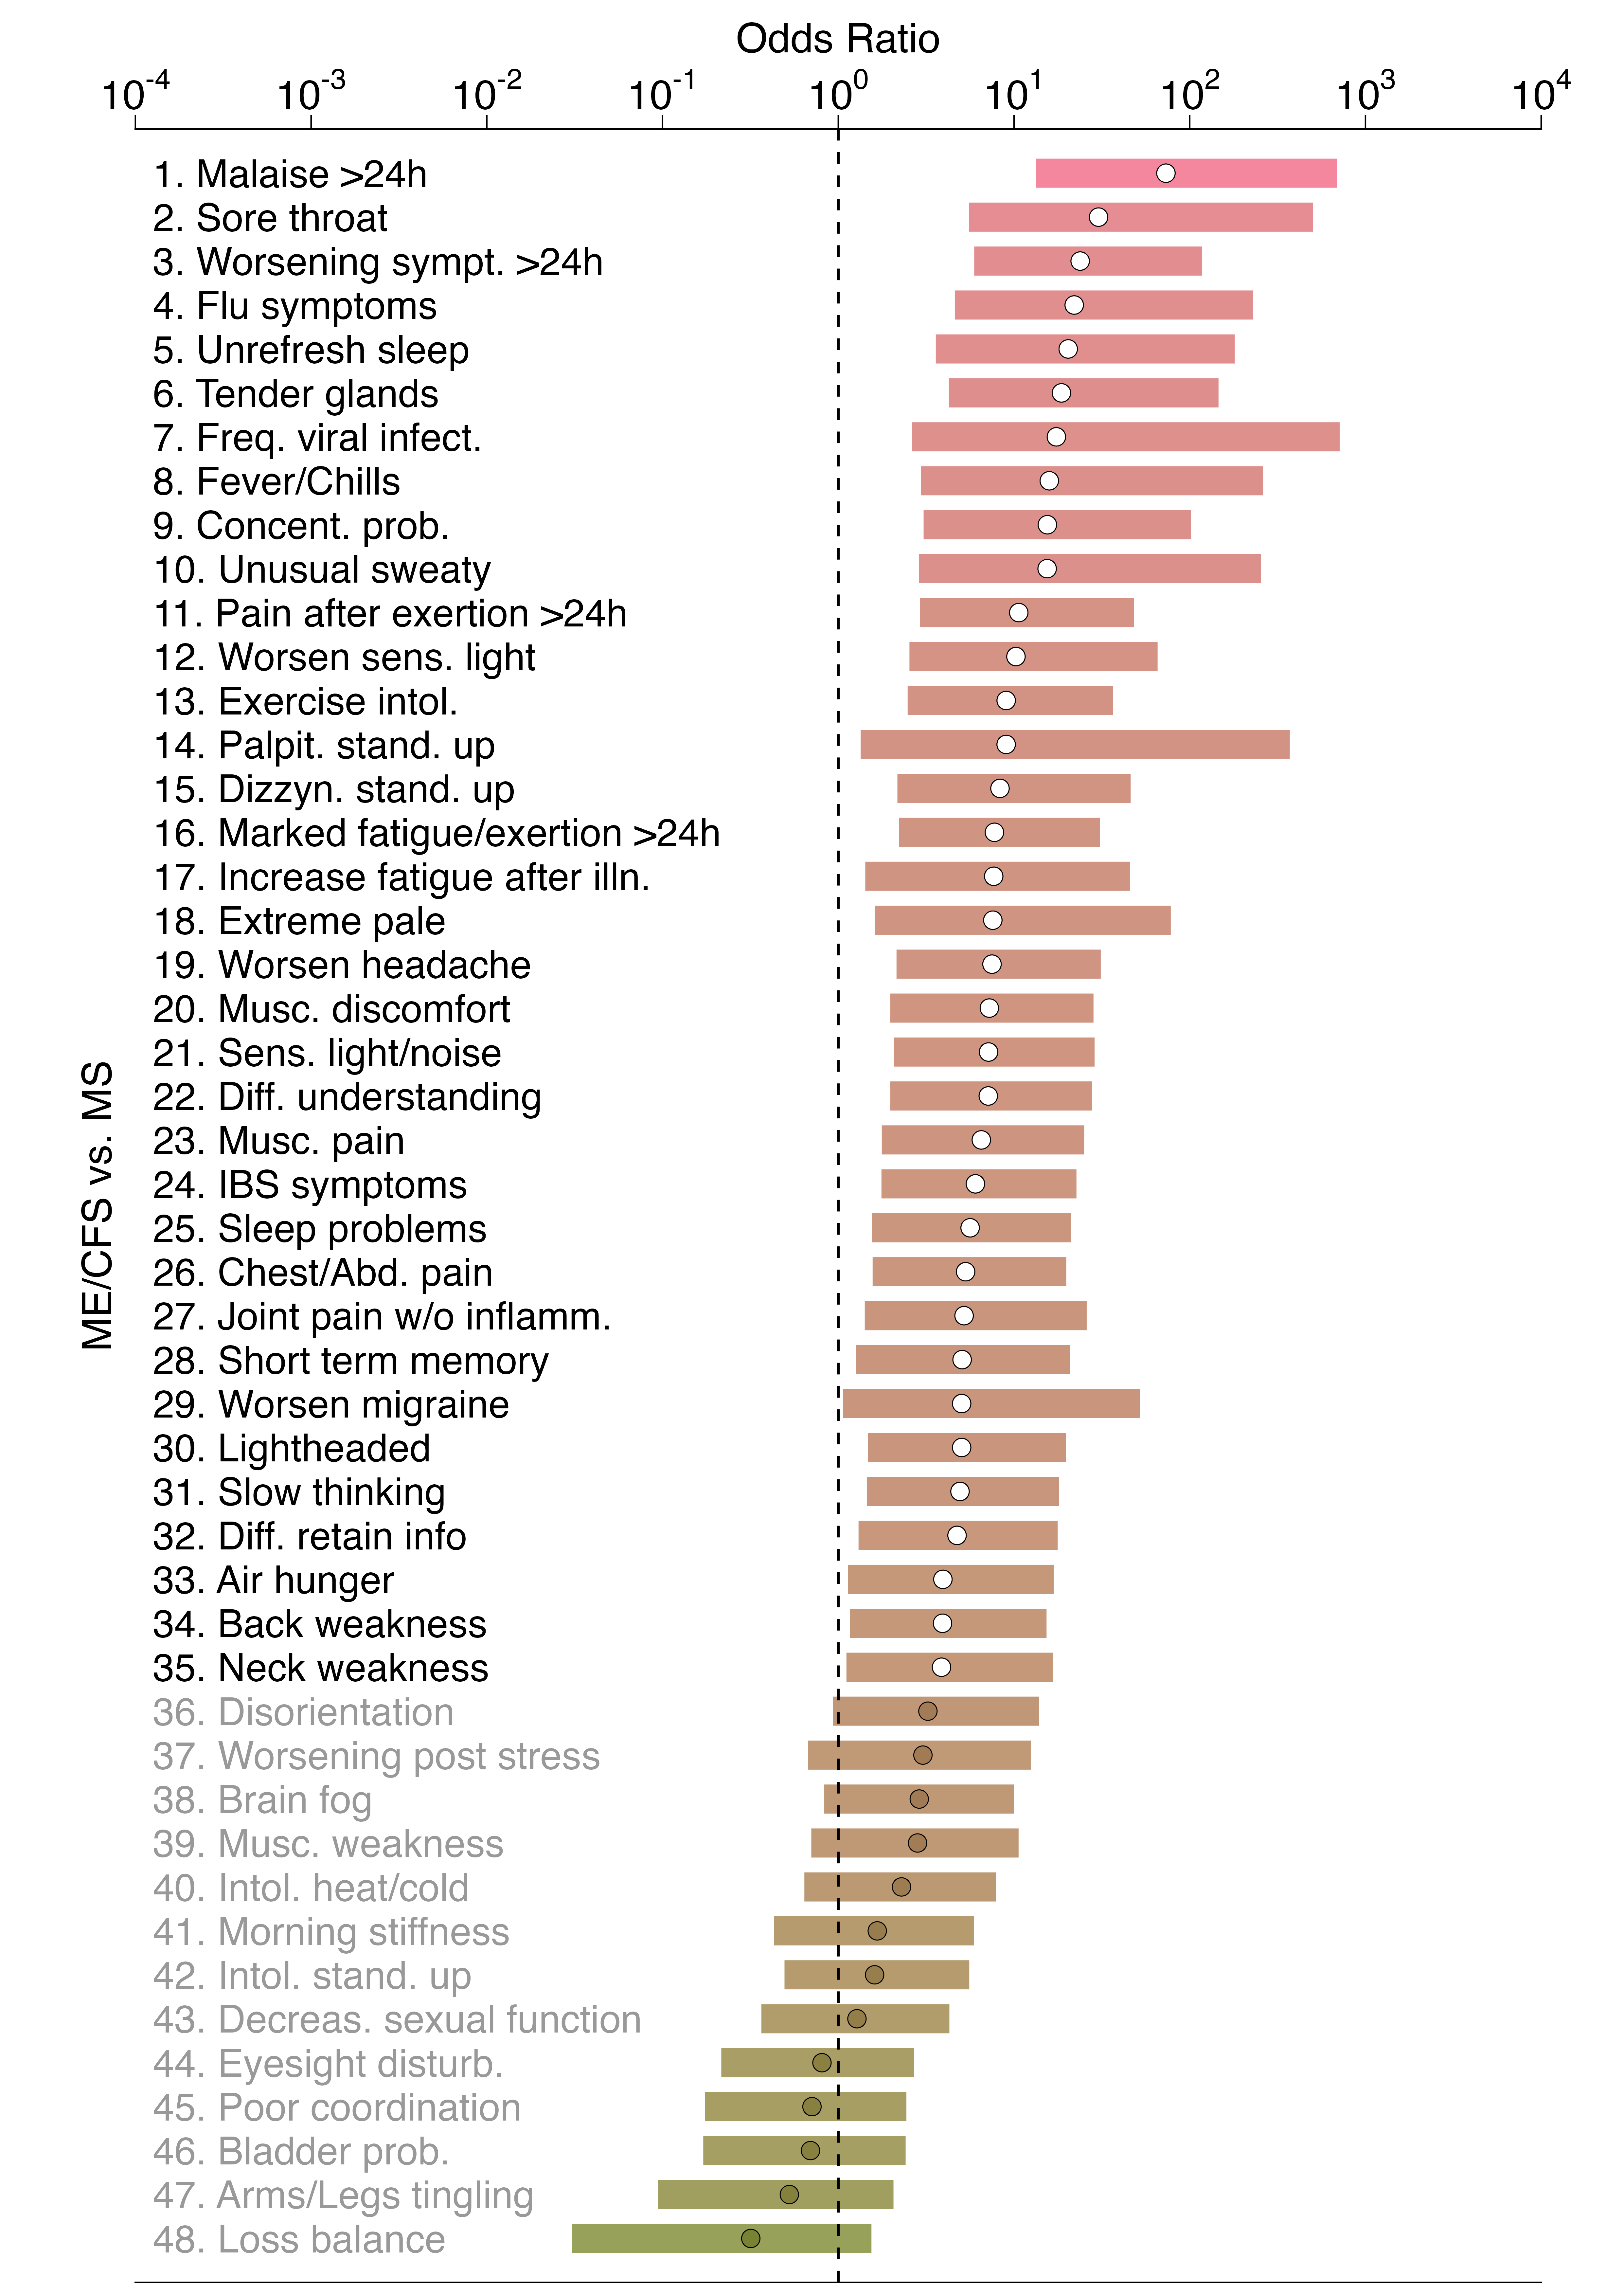
\includegraphics[width=0.85\textwidth]{chapter/2023-sym-and-herpesvirus/figures/fig1-age-adj-or-cfs-all-vs-ms.png}
    \caption[Age-adjusted OR for the presence of each of 48 symptoms when comparing the whole ME/CFS group to the MS group]{Age-adjusted odds ratios (dots) ordered by magnitude and their Bonferroni-adjusted 95\% confidence intervals (horizontal bars) for the presence of each of 48 symptoms when comparing the whole ME/CFS group to the MS group (reference). White-filled dots refer to symptoms where there was evidence of a higher frequency in the ME/CFS group than in the MS group. Grey-filled dots refer to symptoms where there was evidence for the same frequency in both cohorts.}
    \label{fig:fig1-age-adj-or-cfs-all-vs-ms}
\end{figure}
% Figure 1
% Figure~\ref{fig:fig1-age-adj-or-cfs-all-vs-ms}

\begin{figure}
    \centering
    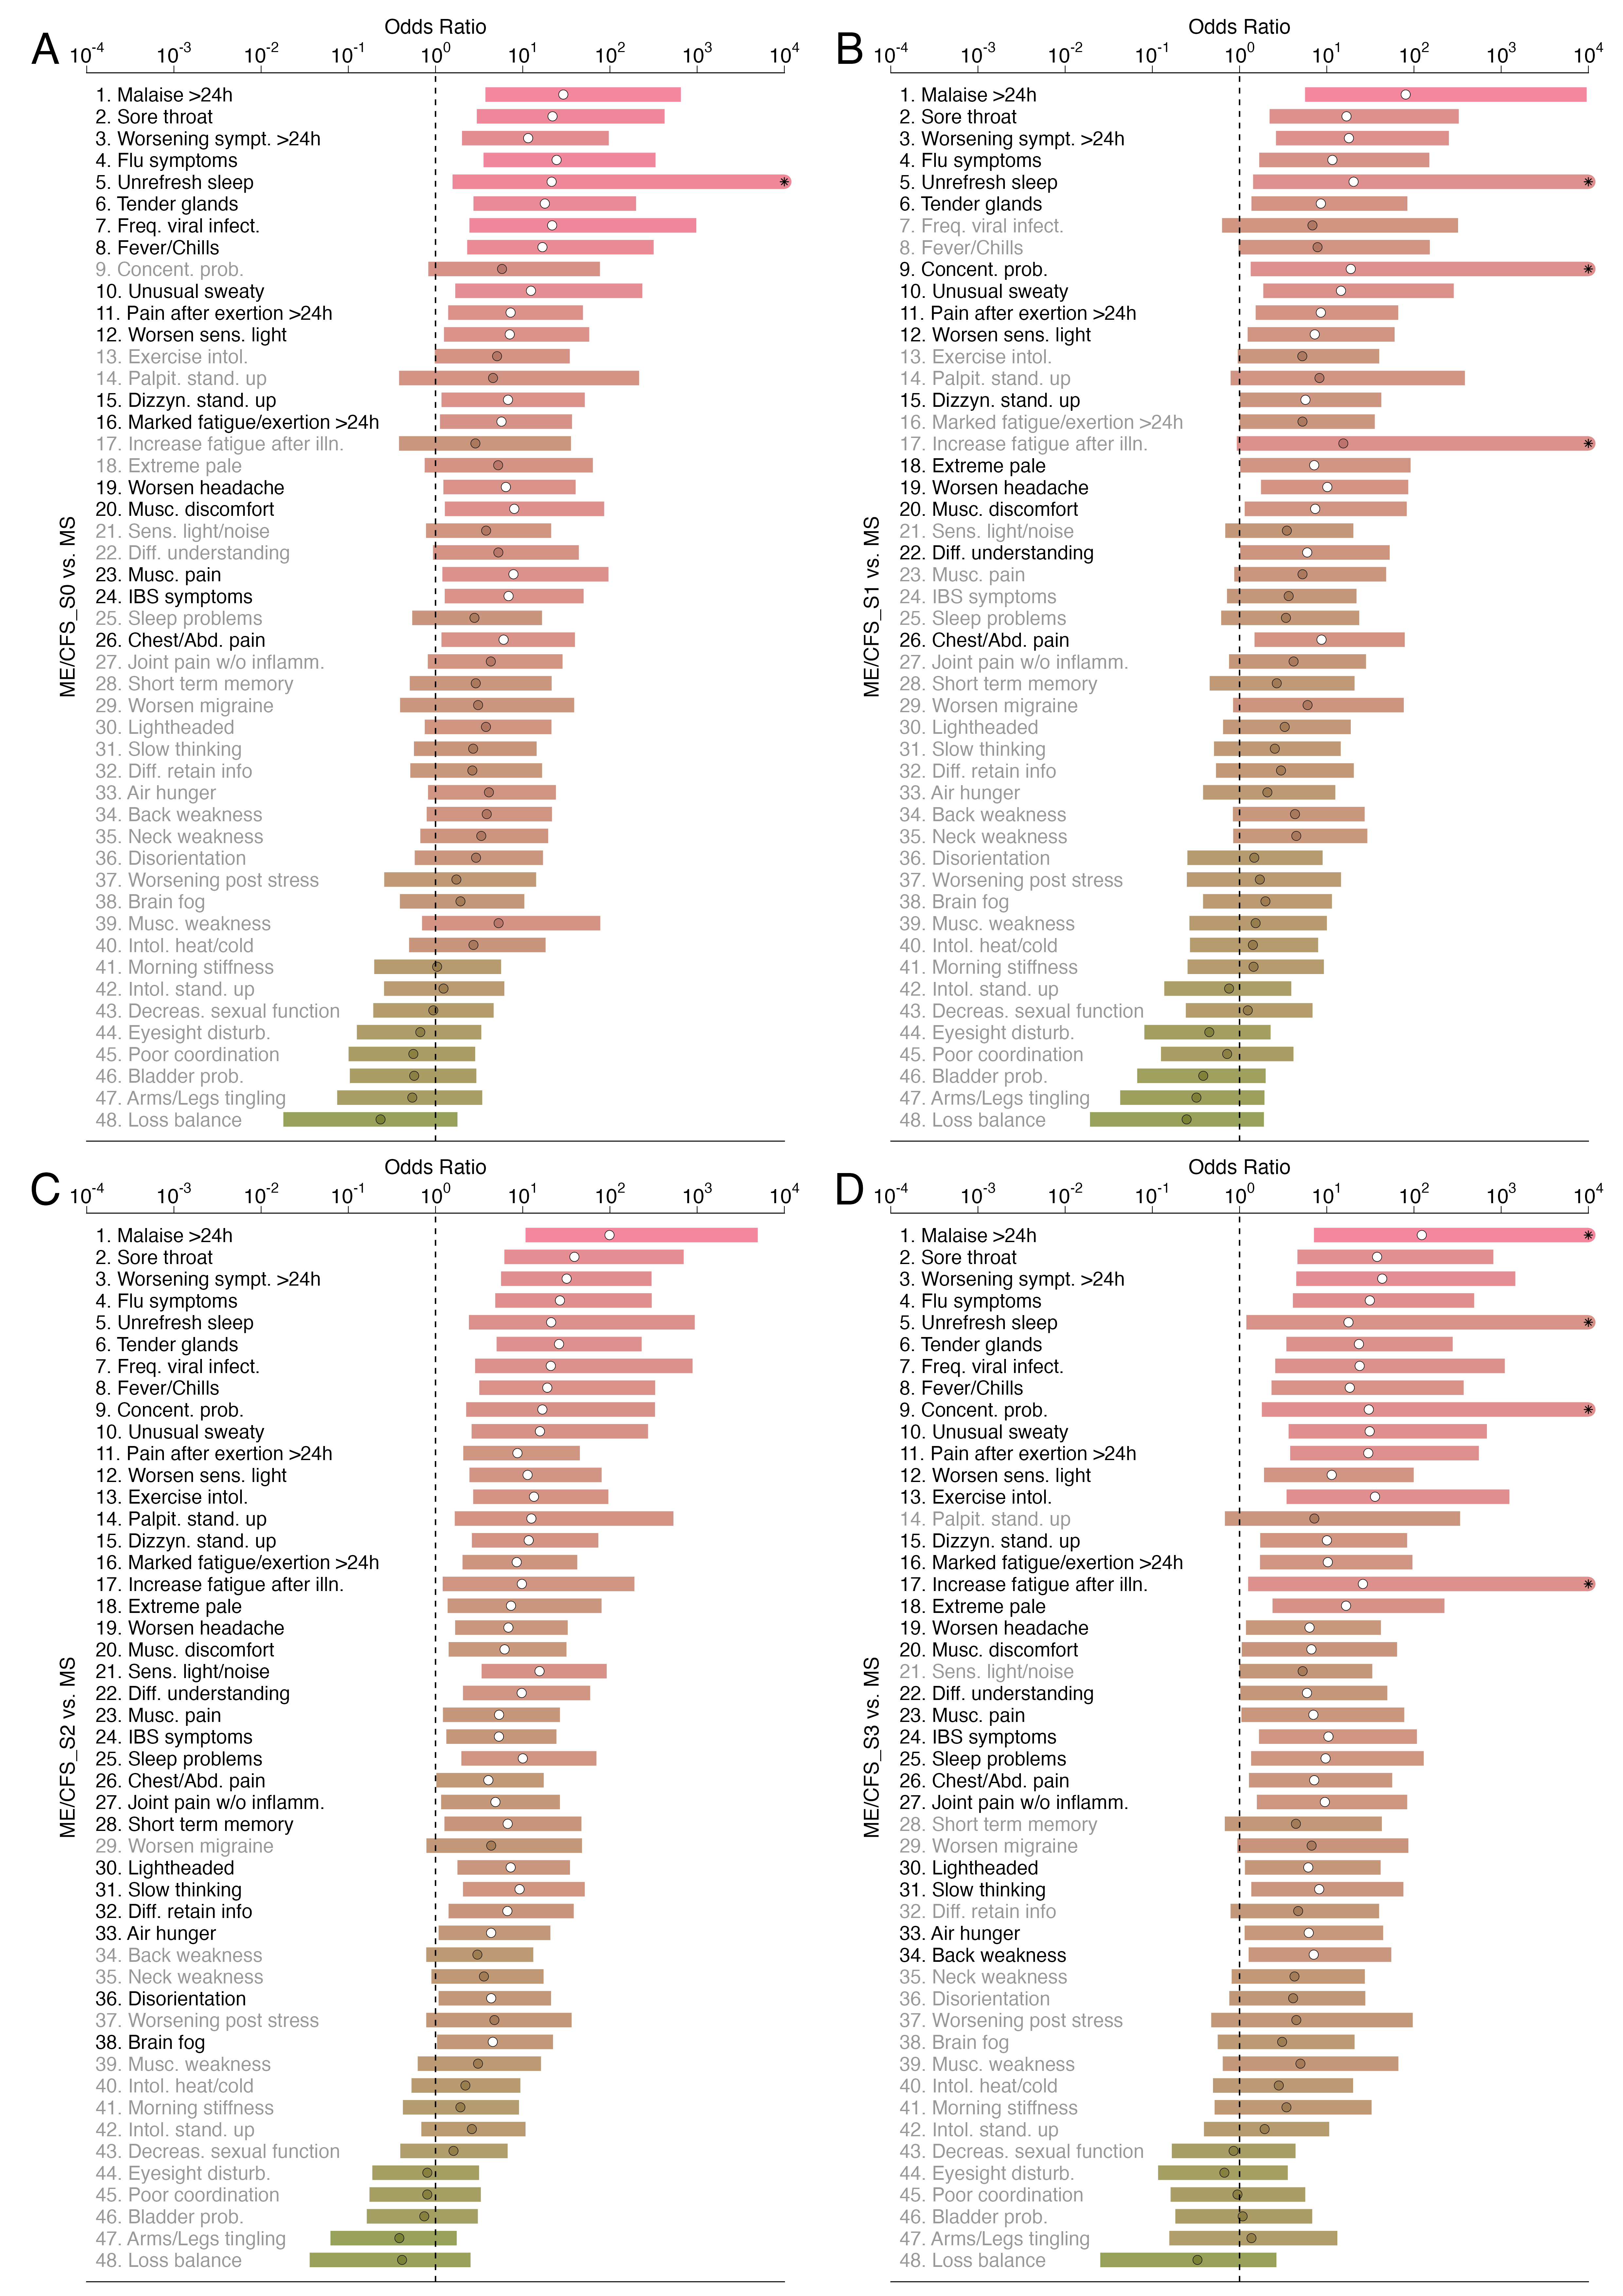
\includegraphics[width=0.87\textwidth]{chapter/2023-sym-and-herpesvirus/figures/fig2-age-adj-or-cfs-other-vs-ms.png}
    \caption[Age-adjusted OR for the presence of each of 48 symptoms when comparing subgroups of ME/CFS to the MS group]{Age-adjusted odds ratios (dots) and their Bonferroni-adjusted 95\% confidence intervals (horizontal bars) for the presence of each of 48 symptoms when comparing ME/CFS\_S0 (A), ME/CFS\_S1 (B), ME/CFS\_S2 (C), and ME/CFS\_S3 (D) to the MS group. The ``${\ast}$'' symbol in some of the bars denotes an upper limit beyond the maximum value used for the $xx$ axis. See Figure~\ref{fig:fig1-age-adj-or-cfs-all-vs-ms} legend for further information.}
    \label{fig:fig2-age-adj-or-cfs-other-vs-ms}
\end{figure}
% Figure 2
% Figure~\ref{fig:fig2-age-adj-or-cfs-other-vs-ms}

\clearpage

%%%%%%%%%%%%%%%%%%%%%%%%%%%%%%%%%%%%%%%%%%%%%%%%%%%%%%%%%%%%%%%%%%%%%%%%
\subsection{Univariate analysis of herpesvirus IgG antibody data}

As stated in the Introduction, EBV and HHV6 infections are thought to be at the origin and a risk factor for both MS \citep{lundstrom2022HumanHerpesvirus, soldan2023EpsteinBarr} and ME/CFS \citep{ruiz-pablos2021EpsteinBarrVirus}. Given this evidence, one could hypothesise that IgG antibody concentrations related to these viruses could be elevated in both diseases. In this regard, we previously found evidence for similar seroprevalence to each herpesvirus, including EBV and HHV6, when comparing mild/moderate and severely affected ME/CFS patients, MS patients, and healthy controls \citep{cliff2019CellularImmune}. Similar evidence was found for the respective antibody concentration levels except a higher EBNA1-VCA IgG antibody concentration in the MS cohort.

Here, we repeated a similar analysis using data of seroprevalence and IgG antibody concentration levels for 5 study groups to test whether a disease-trigger stratification of the ME/CFS group could provide additional information (Table~\ref{tab:tab2-igg-antibodies.description} and Supplementary Figure~\ref{appendix:figa1-quantitative-serology}). Interestingly, the most significant differences remained to be related to both EBV-related IgG antibodies. These differences were in part driven by a higher seroprevalence or a higher median IgG antibody concentration in the MS group, even when compared to the ME/CFS\_S3 group where confirmed EBV infections were reported to be the cause of the disease \citep{domingues2021HerpesvirusesSerologya}. Therefore, our re-analysis using a different ME/CFS patient's stratification was once again against the prior expectation that IgG antibody concentrations related to different herpesviruses are equivalent in ME/CFS and MS.

% Supplementary Figure 1
% Supplementary Figure~\ref{appendix:figa1-quantitative-serology}

\begin{table}[h]
    \centering
    \caption[Seroprevalence, median concentration and respective IQR per study group and herpesvirus IgG antibody]{Seroprevalence (SeroP, in percentage), median concentration and the respective IQR per study group and herpesvirus IgG antibody, where p-value refers to the Pearson's $\chi^2$ test for seroprevalence-based analysis and the Kruskal-Wallis test for the corresponding quantitative data.}
    \resizebox{\linewidth}{!}{\begin{tblr}{
    row{1} = {m},
    column{1-2} = {l},
    column{3-8} = {c},
    hline{1,16} = {-}{0.08em},
    hline{2} = {-}{0.05em},
}
{Herpesvirus\\(Antigen)} & Analysis & ME/CFS\_S0 & ME/CFS\_S1 & ME/CFS\_S2 & ME/CFS\_S3 & MS & p-value \\
CMV         & SeroP (95\% CI) & 42.9 (27.7; 59.0) & 25.6 (13.5; 41.2) & 37.0 (27.1; 47.7) & 18.8 (8.9; 32.6) & 45.0 (29.3; 61.5) & 0.035 \\
& Median (IQR) & 5.4 (78.5)   & 4.6 (13.3)   & 6 (59.8)     & 5.4 (1.5)    & 5.8 (64.4)   & 0.407 \\
% &  &  &  &  &  &  & \\
EBV (EBNA1) & SeroP (95\% CI) & 71.4 (55.4; 84.3) & 58.1 (42.1; 73.0) & 75.0 (64.9; 83.4) & 75.0 (60.4; 86.4) & 95.0 (83.1; 99.4) & 0.004 \\
& Median (IQR) & 39.3 (17.8)  & 24.6 (17.1)  & 37.2 (23.5)  & 32.9 (26.4)  & 46.9 (17.8)  & 0.006 \\
% &  &  &  &  &  &  & \\
EBV (VCA)   & SeroP (95\% CI) & 88.1 (74.4; 96.0) & 74.4 (58.8; 86.5) & 84.8 (75.8; 91.4) & 95.8 (85.7; 99.5) & 92.5 (79.6; 98.4) & 0.030 \\
& Median (IQR) & 99.4 (64.4)  & 88.0 (64.8)  & 108.9 (49.9) & 129.5 (48.6) & 155.4 (33.8) & 0.003 \\
% &  &  &  &  &  &  & \\
HHV6        & SeroP (95\% CI) & 85.7 (71.5; 94.6) & 90.7 (77.9; 97.4) & 92.4 (84.9; 96.9) & 100.0 (92.6; 100.0) & 90.0 (76.3; 97.2) & 0.146 \\
& Median (IQR) & 38.3 (21.1)  & 42.5 (24.3)  & 47.5 (25.2)  & 43.0 (29.7)  & 43.4 (50.8)  & 0.418 \\
% &  &  &  &  &  &  & \\
HSV1        & SeroP (95\% CI) & 50.0 (34.2; 65.8) & 34.9 (21.0; 50.9) & 43.5 (33.2; 54.2) & 54.2 (39.2; 68.6) & 57.5 (40.9; 73.0) & 0.207 \\
& Median (IQR) & 12.1 (89.5)  & 6.6 (56.5)   & 7.6 (108.8)  & 16.5 (119.7) & 22.6 (109.6) & 0.273 \\
% &  &  &  &  &  &  & \\
HSV2        & SeroP (95\% CI) & 50.0 (34.2; 65.8) & 30.2 (17.2; 46.6) & 35.9 (26.1; 46.5) & 45.8 (31.4; 60.8) & 40.0 (24.9; 56.7) & 0.309 \\
& Median (IQR) & 12.2 (61.4)  & 5.0 (33.5)   & 4.1 (45.0)   & 6.2 (41.8)   & 8.1 (41.8)   & 0.650 \\
% &  &  &  &  &  &  & \\
VZV         & SeroP (95\% CI) & 95.2 (83.8; 99.4) & 93.0 (80.9; 98.5) & 100.0 (96.1; 100.0) & 97.9 (88.9; 99.9) & 97.5 (86.8; 99.9) & 0.169 \\
& Median (IQR) & 129.5 (46.2) & 119.7 (20.8) & 135.7 (48.4) & 142.2 (35.8) & 156.2 (36.7) & 0.069 \\
\end{tblr}}
    \label{tab:tab2-igg-antibodies.description}
\end{table}
% Table 2
% Table~\ref{tab:tab2-igg-antibodies.description}

In agreement with our previous analysis when we compared ME/CFS subgroups to MS \citep{domingues2021HerpesvirusesSerologya}, differences in CMV seroprevalence groups were in the vicinity of statistical significance. This result was due to lower seroprevalences to this virus in ME/CFS\_S1 and ME/CFS\_S3. For the remaining herpesvirus antibodies, there were no significant differences among the study groups in terms of seroprevalence or IgG antibody concentrations.

We extended this analysis with the objective of discriminating patients with MS from healthy controls combining these data with a ROC curve approach (Supplementary Table~\ref{appendix:taba3-models-auc-optimal-cutoff-ms}). The most significant AUC result was found for the antibodies against EBV-VCA. In this case, the respective antibody concentrations were significantly increased in patients with MS. The estimate of AUC was 0.641 (95\% CI = [0.538, 0.744)) with an optimal sensitivity and specificity of approximately 0.650. Another significant result was found for antibodies against HSV1 (AUC = 0.626; 95\% CI = [0.531, 0.721]). Interestingly, these antibodies were in higher concentrations in healthy controls than in MS patients. The corresponding sensitivity and specificity were estimated at 0.950 and 0.327, respectively. This result indicated that MS patients are well characterised by a low HSV1 antibody concentration. The data from the remaining antibodies did not provide any evidence for a significant result.

% Supplementary Table 3
% Supplementary Table~\ref{appendix:taba3-models-auc-optimal-cutoff-ms}

We then performed a classification exercise of each subgroup of ME/CFS patients using patients with MS as the control group (Table~\ref{tab:tab3-models-auc-optimal-cutoff-se-sp}). In general, the MS cohort tended to have higher antibody concentrations than the ME/CFS patients, irrespective of the herpesvirus under analysis apart from a single exception, ME/CFS\_S0 vs. MS for CMV. However, the classification power of each antibody was not significant as illustrated by the 95\% confidence interval for the AUC that contained the value 0.50. The most optimistic scenarios were observed for the pairwise comparisons involving the EBV-related antigens. In particular, the best classification was obtained for ME/CFS\_S1 vs. MS for EBNA1 (AUC = 0.741; 95\% CI = [0.634, 0.848]). In this case, the sensitivity and specificity were estimated at 0.465 and 0.950, respectively, using a cutoff of 20.0 U/ml. These estimates suggested that high antibody concentrations to this EBV antigen were able to discriminate MS patients almost perfectly. However, the same could not be said for detecting cases from this ME/CFS subgroup.

\begin{table}
    \centering
    \caption[Area under the Receiver Operating Characteristic curve and its 95\% confidence interval, optimal cutoff and associated sensitivity and specificity to discriminate ME/CFS\_S0, ME/CFS\_S1, ME/CFS\_S2, ME/CFS\_S3 subgroups from patients with multiple sclerosis used as controls]{Area under the Receiver Operating Characteristic curve (AUC) and its 95\% confidence interval (CI), optimal cutoff and associated sensitivity (Se) and specificity (Sp) to discriminate ME/CFS\_S0, ME/CFS\_S1, ME/CFS\_S2, ME/CFS\_S3 subgroups (cases) from patients with multiple sclerosis (MS) used as controls. In the Direction column, the symbols ``{>}'' and ``{<}'' represent higher value in MS cases than in healthy controls and vice-versa, respectively. In the Cutoff column, the p-value within parenthesis is associated with the Pearson's $\chi^2$ test for $2 \times 2$ tables after adjusting for an FDR of 5\%. In the AUC column, the symbol ``{$\ast$}'' denote the cases where there was evidence of an AUC different from 0.50 (random guess).}
    \resizebox{0.98\linewidth}{!}{\begin{tblr}{
    row{1} = {m},
    column{1} = {l},
    column{2,3,4,5,6,7} = {c},
    hline{1,36} = {-}{0.08em},
    hline{2} = {-}{0.05em},
}
{Herpesvirus\\(Antigen)} & Comparison ($vs.$ MS) & Direction & {AUC (95\% CI)} & {Cutoff in U/ml\\(p-value)} & Se & Sp \\
CMV & ME/CFS\_S0 & $\text{controls} < \text{cases}$ & 0.551 (0.421; 0.680) & 2.845 (0.0214) & 0.952 & 0.325 \\
    & ME/CFS\_S1 & $\text{controls} > \text{cases}$ & 0.547 (0.418; 0.677) & 29.21 (0.0701) & 0.791 & 0.425 \\
    & ME/CFS\_S2 & $\text{controls} < \text{cases}$ & 0.507 (0.389; 0.624) & 194.91 (0.0256) & 0.000 & 0.900 \\
    & ME/CFS\_S3 & $\text{controls} > \text{cases}$ & 0.545 (0.413; 0.678) & 58.755 (0.0028) & 0.938 & 0.375 \\
 &  &  &  &  &  & \\
EBV (EBNA1) & ME/CFS\_S0 & $\text{controls} > \text{cases}$ & 0.590 (0.463; 0.716) & 15.415 (0.0257) & 0.286 & 0.950 \\
    & ME/CFS\_S1 & $\text{controls} > \text{cases}$ & 0.741 (0.634; 0.848)$\ast$ & 20.035 (0.0004) & 0.465 & 0.950 \\
    & ME/CFS\_S2 & $\text{controls} > \text{cases}$ & 0.602 (0.505; 0.700)$\ast$ & 20.505 (0.0035) & 0.359 & 0.950 \\
    & ME/CFS\_S3 & $\text{controls} > \text{cases}$ & 0.621 (0.503; 0.739)$\ast$ & 19.985 (0.0028) & 0.396 & 0.950 \\
&  &  &  &  &  & \\
EBV (VCA) & ME/CFS\_S0 & $\text{controls} > \text{cases}$ & 0.668 (0.550; 0.787)$\ast$ & 132.96 (0.0257) & 0.643 & 0.675 \\
    & ME/CFS\_S1 & $\text{controls} > \text{cases}$ & 0.695 (0.580; 0.811)$\ast$ & 71.435 (0.0029) & 0.442 & 0.900 \\
    & ME/CFS\_S2 & $\text{controls} > \text{cases}$ & 0.645 (0.543; 0.746)$\ast$ & 150.345 (0.0144) & 0.707 & 0.575 \\
    & ME/CFS\_S3 & $\text{controls} > \text{cases}$ & 0.566 (0.443; 0.690) & 139.315 (0.0687) & 0.583 & 0.650 \\
&  &  &  &  &  & \\
HHV6 & ME/CFS\_S0 & $\text{controls} > \text{cases}$ & 0.590 (0.465; 0.714) & 78.105 (0.0374) & 0.881 & 0.350 \\
    & ME/CFS\_S1 & $\text{controls} > \text{cases}$ & 0.558 (0.429; 0.687) & 103.94 (0.0057) & 1.000 & 0.225 \\
    & ME/CFS\_S2 & $\text{controls} > \text{cases}$ & 0.518 (0.403; 0.632) & 130.625 (0.0256) & 0.978 & 0.150 \\
    & ME/CFS\_S3 & $\text{controls} > \text{cases}$ & 0.520 (0.391; 0.649) & 91.82 (0.0271) & 0.938 & 0.275 \\
&  &  &  &  &  & \\
HSV1 & ME/CFS\_S0 & $\text{controls} > \text{cases}$ & 0.579 (0.454; 0.704) & 2.14 (0.0371) & 0.167 & 1.000 \\
    & ME/CFS\_S1 & $\text{controls} > \text{cases}$ & 0.635 (0.513; 0.756)$\ast$ & 2.84 (0.0104) & 0.256 & 0.975 \\
    & ME/CFS\_S2 & $\text{controls} > \text{cases}$ & 0.596 (0.497; 0.696) & 2.755 (0.0303) & 0.196 & 0.975 \\
    & ME/CFS\_S3 & $\text{controls} > \text{cases}$ & 0.550 (0.429; 0.671) & 2.8 (0.0182) & 0.250 & 0.975 \\
&  &  &  &  &  & \\
HSV2 & ME/CFS\_S0 & $\text{controls} < \text{cases}$ & 0.557 (0.432; 0.683) & 231.395 (0.0737) & 0.119 & 1.000 \\
    & ME/CFS\_S1 & $\text{controls} > \text{cases}$ & 0.536 (0.409; 0.663) & 6.81 (0.1600) & 0.628 & 0.55 \\
    & ME/CFS\_S2 & $\text{controls} > \text{cases}$ & 0.520 (0.410; 0.629) & 7.03 (0.1343) & 0.609 & 0.550 \\
    & ME/CFS\_S3 & $\text{controls} > \text{cases}$ & 0.527 (0.402; 0.651) & 2.895 (0.1341) & 0.771 & 0.400 \\
&  &  &  &  &  & \\
VZV & ME/CFS\_S0 & $\text{controls} > \text{cases}$ & 0.596 (0.472; 0.721) & 141.005 (0.0737) & 0.571 & 0.650 \\
    & ME/CFS\_S1 & $\text{controls} > \text{cases}$ & 0.667 (0.548; 0.786)$\ast$ & 139.495 (0.0025) & 0.744 & 0.650 \\
    & ME/CFS\_S2 & $\text{controls} > \text{cases}$ & 0.532 (0.418; 0.646) & 148.24 (0.5054) & 0.554 & 0.550 \\
    & ME/CFS\_S3 & $\text{controls} > \text{cases}$ & 0.546 (0.421; 0.672) & 180.995 (0.0981) & 0.792 & 0.400
 \end{tblr}}
    \label{tab:tab3-models-auc-optimal-cutoff-se-sp}
\end{table}
% Table 3
% Table~\ref{tab:tab3-models-auc-optimal-cutoff-se-sp}

ME/CFS\_S1 seemed the most different one from the MS group in terms of herpesvirus IgG antibodies (Table~\ref{tab:tab3-models-auc-optimal-cutoff-se-sp}). This interpretation was supported by a significant AUC for antibodies against EBNA1 (as reported above), EBV-VCA (AUC = 0.695; 95\% CI = [0.580, 0.811]; Se = 0.442, Sp = 0.900), HSV1 (AUC = 0.635; 95\% CI = [0.513, 0.756]; Se = 0.256, Sp = 0.975), and VZV (AUC = 0.667; 95\% CI = [0.548, 0.786]; Se = 0.744, Sp = 0.630). This result suggested that combining data from multiple antibodies could help discriminating these two groups of patients.

%%%%%%%%%%%%%%%%%%%%%%%%%%%%%%%%%%%%%%%%%%%%%%%%%%%%%%%%%%%%%%%%%%%%%%%%
\subsection{Combined analysis of IgG antibody data using an SL algorithm}

In this step of the analysis, we integrated all IgG antibody data in several classifiers to distinguish patients of each ME/CFS subgroup from patients with MS. For each pairwise comparison, these classifiers were then assembled into a final classifier using an SL algorithm (Figure~\ref{fig:fig3-roc-curves-sl-algorithm}).

This combined data analysis provided evidence for an AUC significantly different from 0.5 (random guess) for ME/CFS\_S0 (AUC = 0.658; 95\% CI = [0.536, 0.779]), ME/CFS\_S1 (AUC = 0.731; 95\% CI = [0.622, 0.841]), and ME/CFS\_S3 (AUC = 0.707; 95\% CI = [0.599, 0.816]) subgroups using the MS group as a control. The highest sensitivity was obtained for the ME/CFS\_S2 group (0.772), but at the cost of a poor specificity related to the MS group (0.075) (Figure~\ref{fig:fig3-roc-curves-sl-algorithm}). The most balanced sensitivity and specificity estimates were observed for ME/CFS\_S0 vs. MS (0.619 and 0.725, respectively). In the remaining pairwise comparisons (ME/CFS\_S1 and ME/CFS\_S3), there was evidence of a high specificity (higher than 0.90) but a modest sensitivity (up to 0.512).

\clearpage

\begin{figure}[ht]
    \centering
    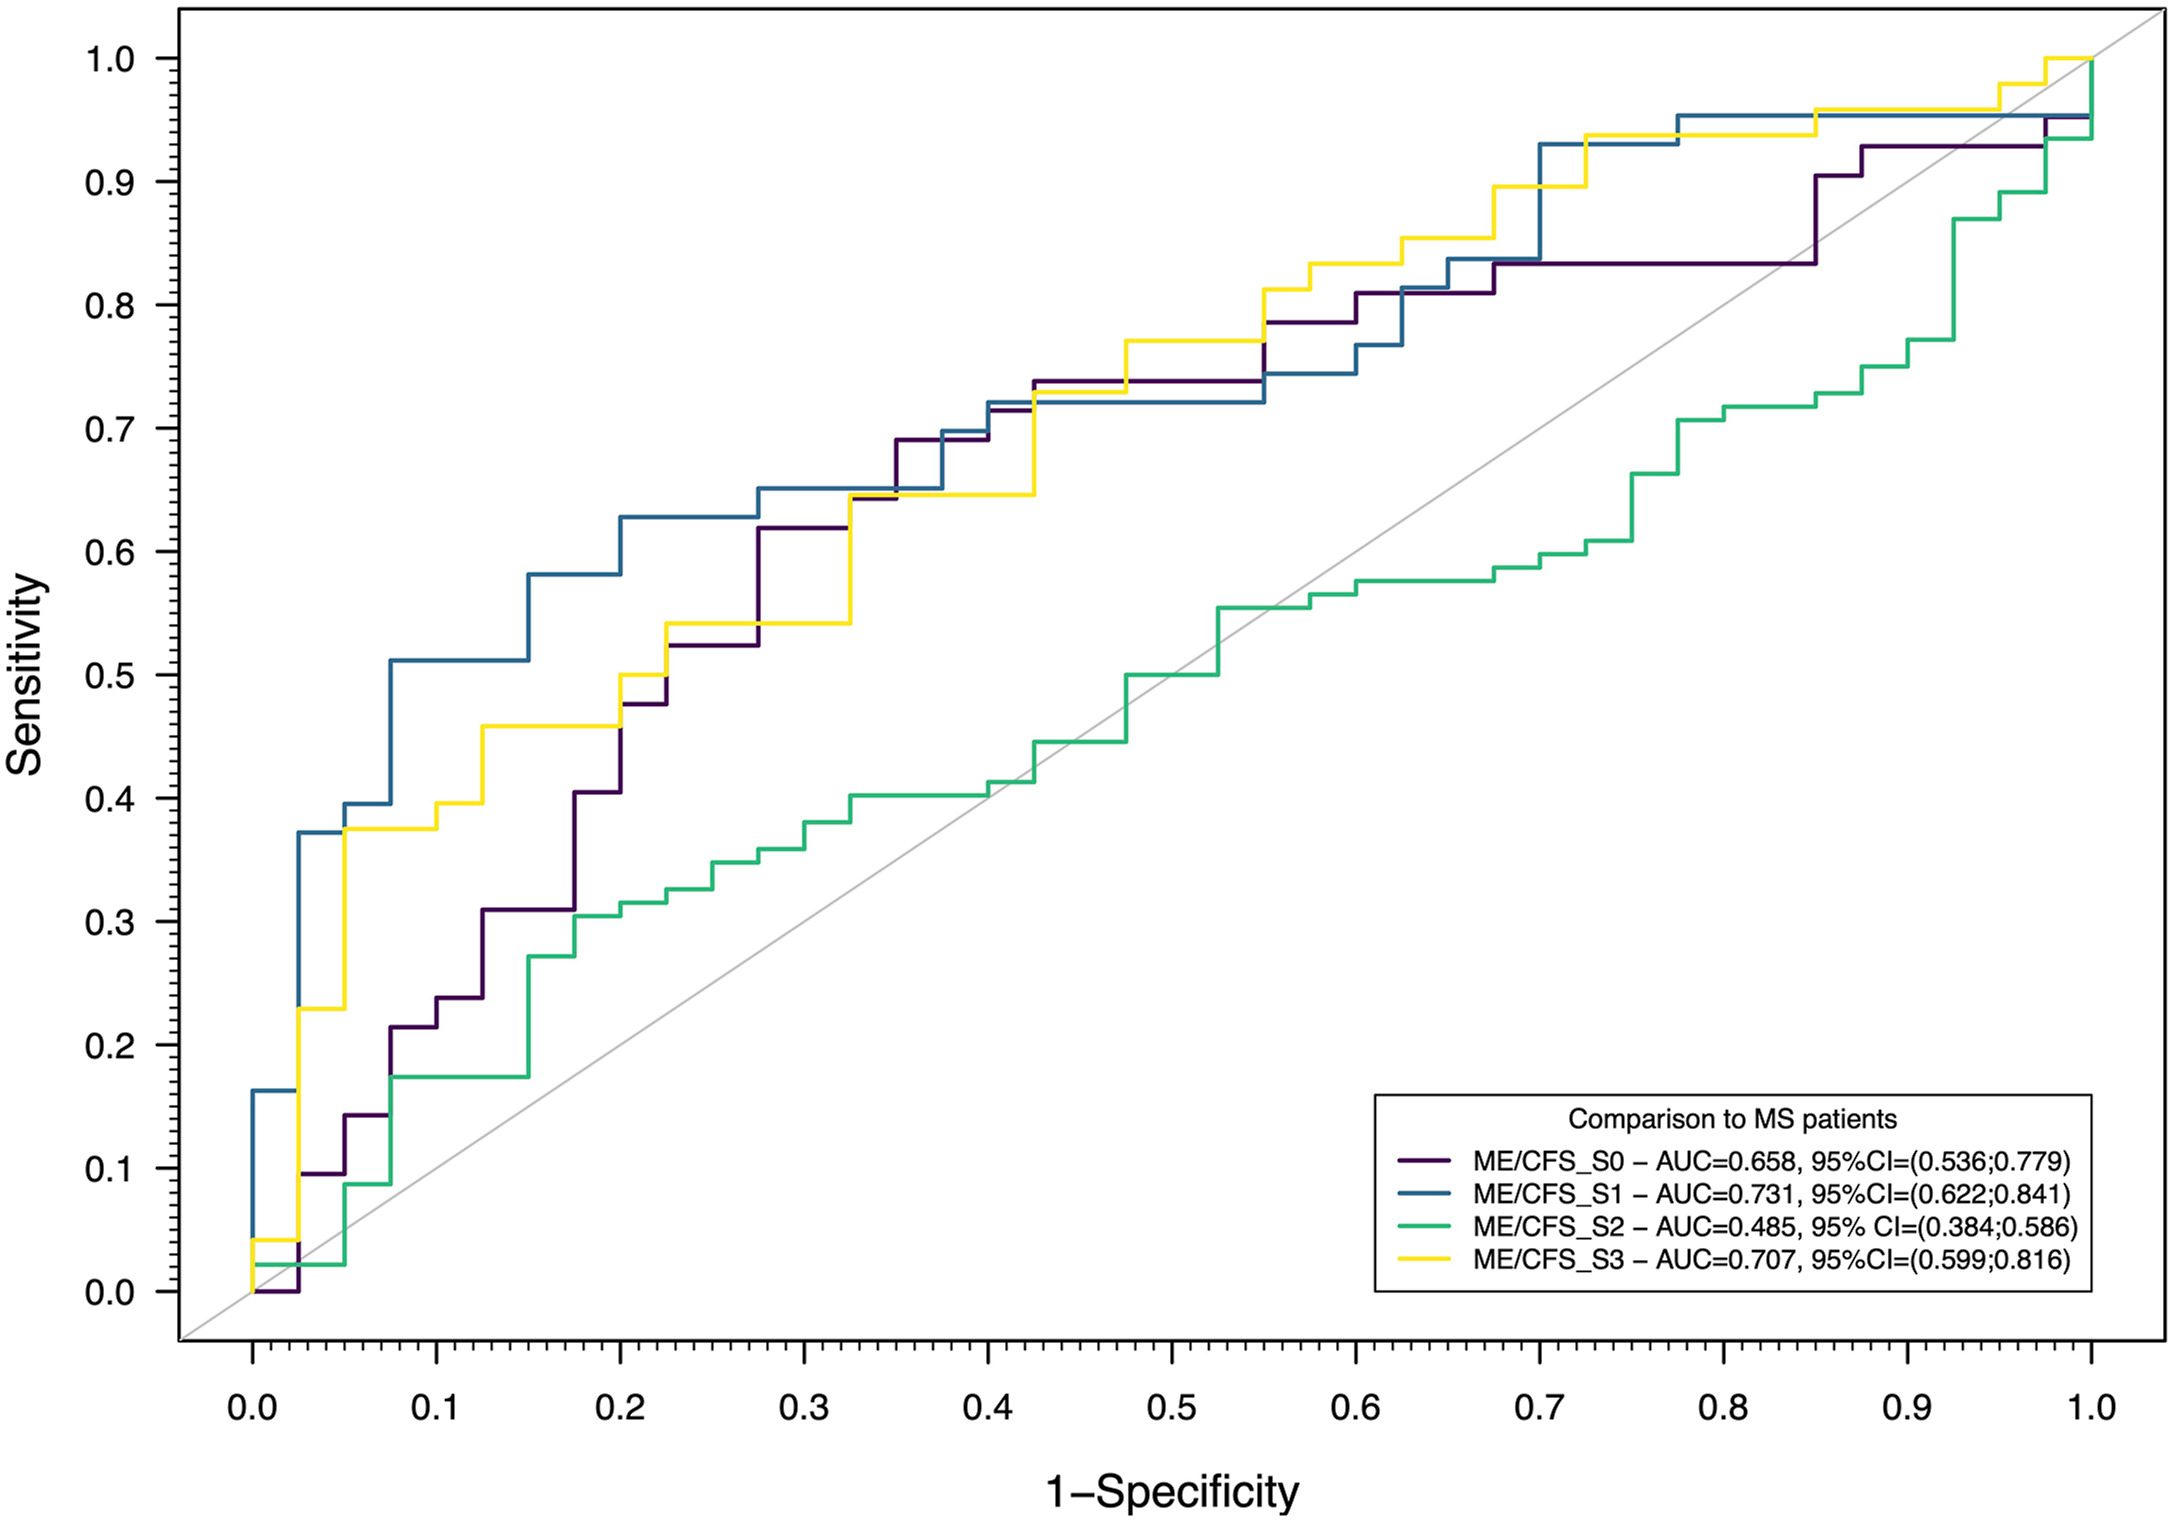
\includegraphics[width=0.85\textwidth]{chapter/2023-sym-and-herpesvirus/figures/fig3-roc-curves-sl-algorithm.jpg}
    \caption[ROC curves for the predictions based on an SL algorithm trained with 4 different classifiers and 10-fold cross-validation using antibody data and patients with MS as the controls]{ROC curves for the predictions based on an SL algorithm trained with 4 different classifiers (Elastic-Net Logistic Regression, Linear Discriminant Analysis, Quadratic Discriminant Analysis, and Random Forest) and 10-fold cross-validation using antibody data and patients with MS as the controls. Optimal sensitivities and specificities were estimated at 0.619 and 0.725 for ME/CFS\_S0, 0.512 and 0.925 for ME/CFS\_S1, 0.772 and 0.075 for ME/CFS\_S2, 0.375 and 0.950 for ME/CFS\_S3, when compared to the MS group.}
    \label{fig:fig3-roc-curves-sl-algorithm}
\end{figure}
% Figure 3
% Figure~\ref{fig:fig3-roc-curves-sl-algorithm}

As expected from the analysis based on a single antibody, the best AUC was obtained for the comparison between ME/CFS\_S1 and MS. When compared to the MS group, the probability of having a patient from this ME/CFS subgroup decreased with the antibody concentrations related to different herpesviruses including EBV (Figure~\ref{fig:fig4-smooth-line-approximations}A--G); see the respective probability profiles for the remaining pairwise comparison in Supplementary Figure~\ref{appendix:figa2-ms-vs-s0}, Supplementary Figure~\ref{appendix:figa3-ms-vs-s2}, and Supplementary Figure~\ref{appendix:figa4-ms-vs-s3} (ME/CFS\_S0 vs. MS, ME/CFS\_S2 vs. MS, ME/CFS\_S3 vs. MS, respectively). Note that, given the poor discrimination between ME/CFS\_S2 and MS, the probability profile of having a patient from this ME/CFS subgroup was almost constant across all the herpesviruses antibodies (Supplementary Figure~\ref{appendix:figa3-ms-vs-s2}).
% Supplementary Figure 2
% Supplementary Figure~\ref{appendix:figa2-ms-vs-s0}
% Supplementary Figure 3
% Supplementary Figure~\ref{appendix:figa3-ms-vs-s2}
% Supplementary Figure 4
% Supplementary Figure~\ref{appendix:figa4-ms-vs-s3}


\begin{figure}[h]
    \centering
    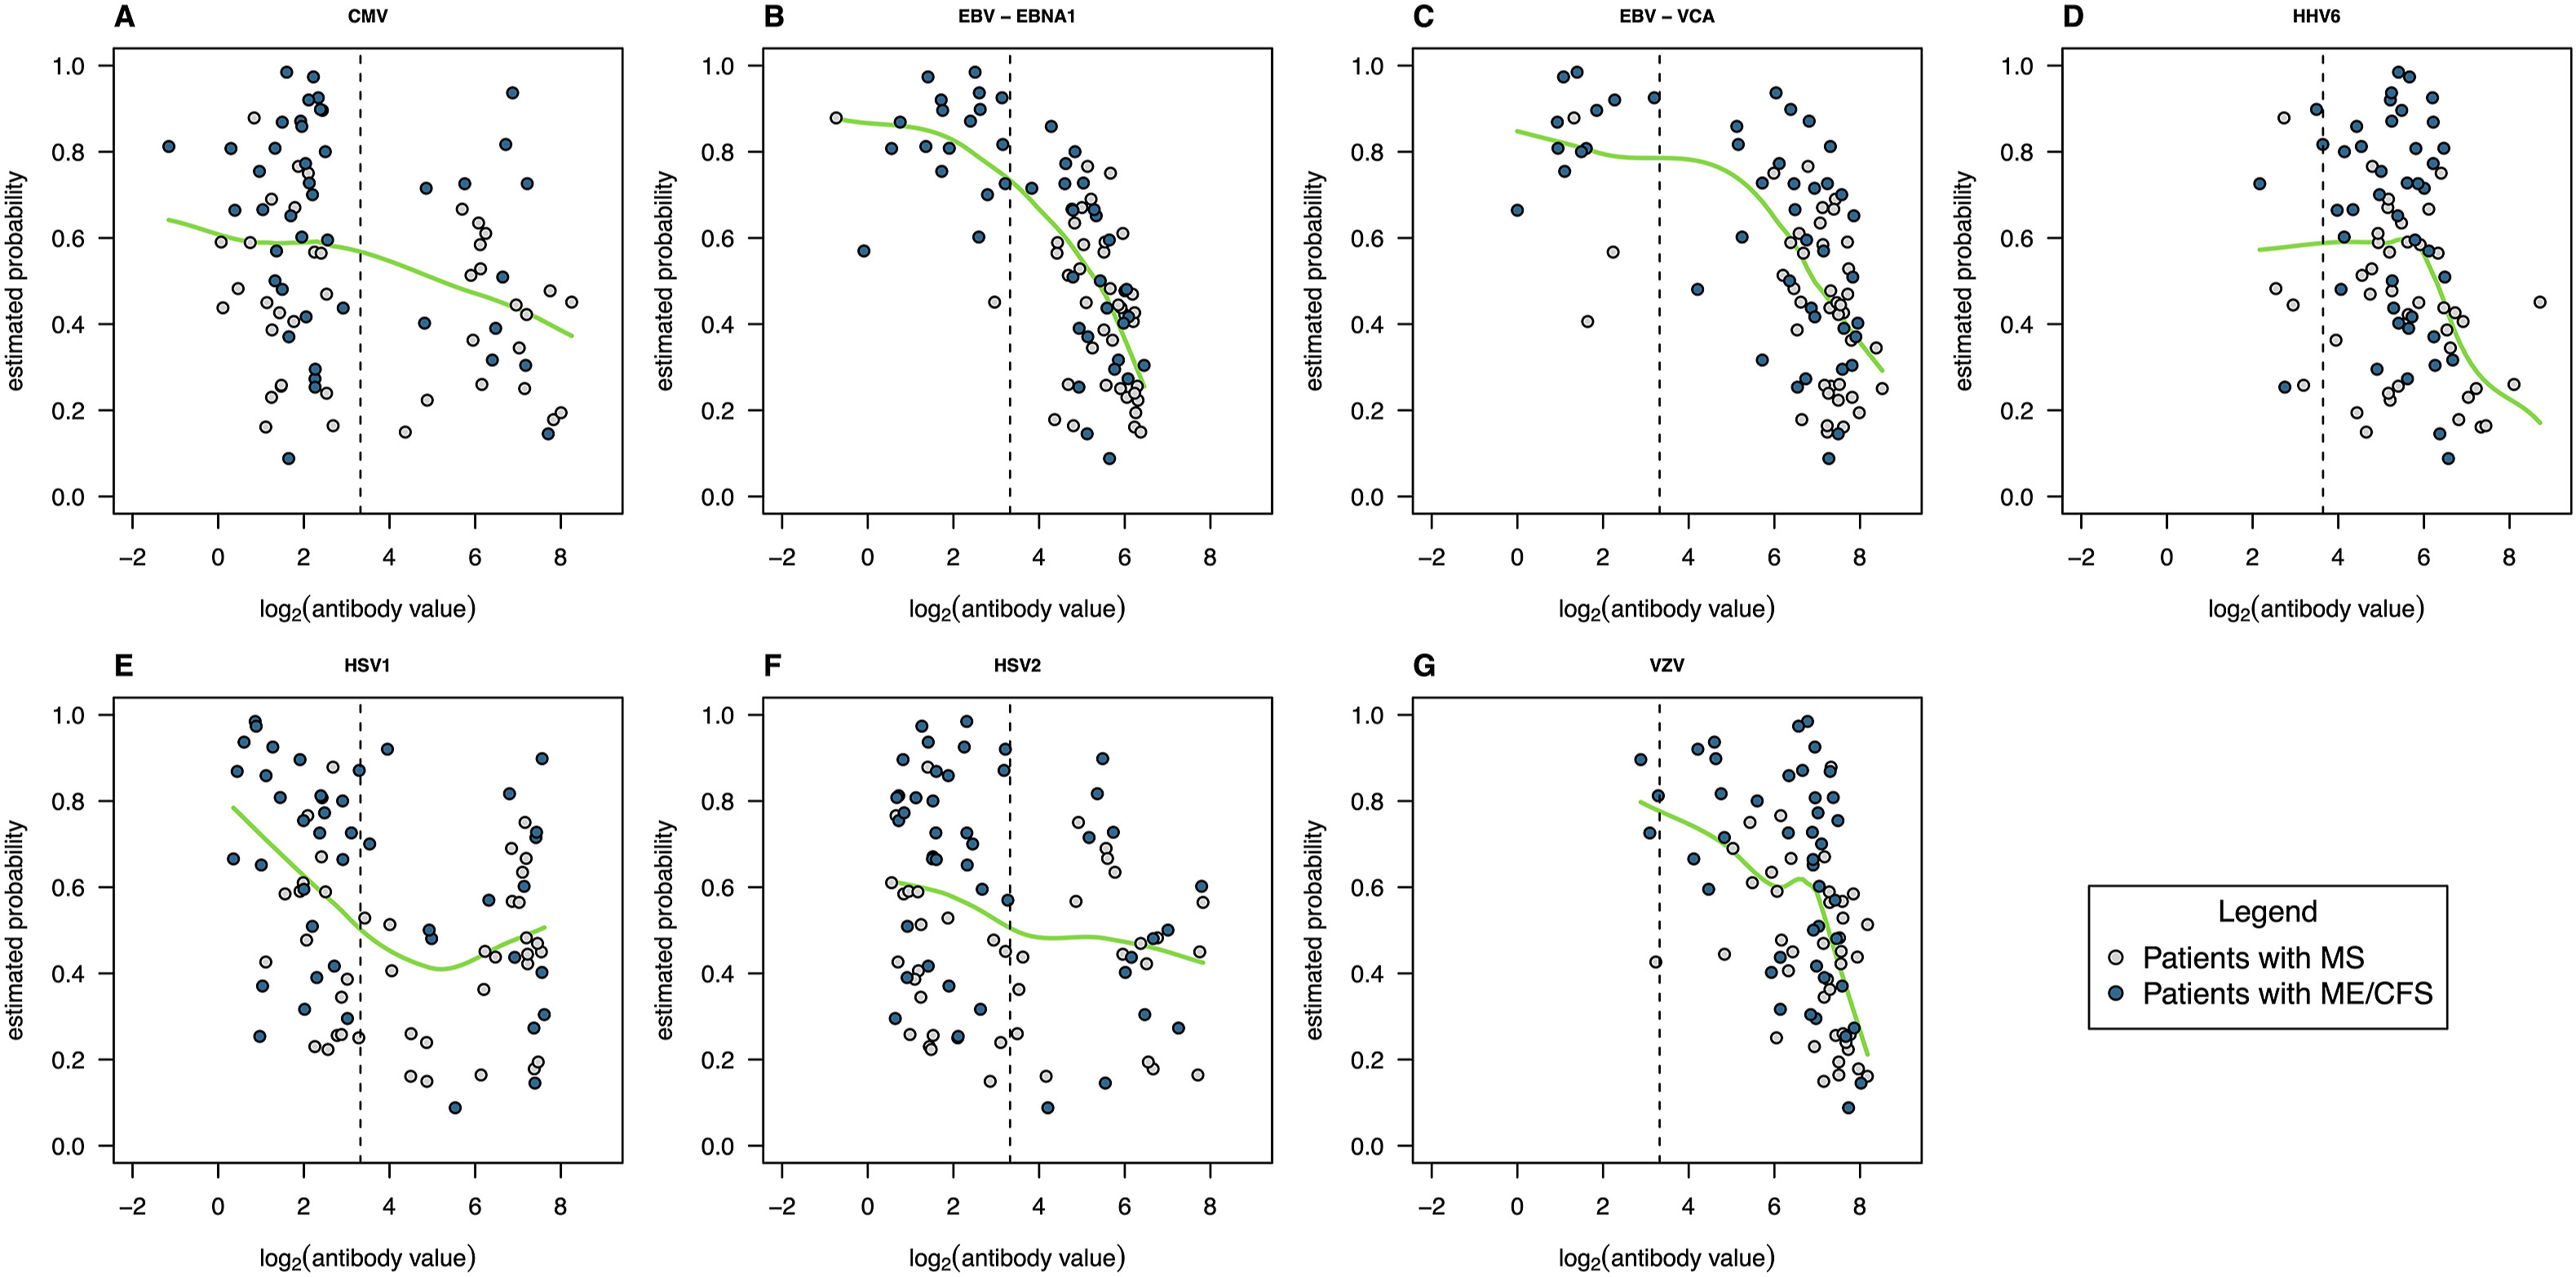
\includegraphics[width=0.9\textwidth]{chapter/2023-sym-and-herpesvirus/figures/fig4-smooth-line-approximations.jpg}
    \caption[Smooth-line approximations of the relationship between $\log_{2}$(antibody concentrations) and SL-estimated probability of ME/CFS\_S1 patient when compared to patients with MS]{Smooth-line approximations (green lines) of the relationship between $\log_{2}$(antibody concentrations) and SL-estimated probability of ME/CFS\_S1 patient when compared to patients with MS (A--CMV, B--EBV-EBNA1, C--EBV-VCA, D--HHV-6, E--HSV1, F--HSV2, G--VZV). In the plots, each dot represents a patient and the vertical dashed line represents the cut-off value for seropositivity according to the respective lab protocol.}
    \label{fig:fig4-smooth-line-approximations}
\end{figure}
% Figure 4
% Figure~\ref{fig:fig4-smooth-line-approximations}

%%%%%%%%%%%%%%%%%%%%%%%%%%%%%%%%%%%%%%%%%%%%%%%%%%%%%%%%%%%%%%%%%%%%%%%%
\subsection{Association analysis between symptomology and herpesvirus IgG antibodies}

Lastly, we correlated the data of presence/absence of each symptom with data of each herpesvirus IgG antibody (Figure~\ref{fig:fig5-association-anslysis-igg-and-cohorts}A--F). In the case of the MS cohort, HHV6 antibody concentration was significantly and negatively associated with difficulties in understanding, and worsening of symptoms after stress. Similar significant negative association was found between CMV IgG antibody concentrations and eyesight disturbances. The only significant positive association was found for EBV-EBNA1 antibody concentrations and bladder problems.

For the overall ME/CFS group, a positive and a negative association reached statistical significance between brain fog and HSV1 IgG antibody concentrations and between chest/abdominal pain and HHV6 antibody concentrations, respectively. These significant associations could not be confirmed by the subsequent subgroup analysis. For the ME/CFS\_S0 subgroup, two significant negative associations were found (neck weakness/HSV1 antibody concentrations and fever chills/EBV-VCA antibody concentrations). In the ME/CFS\_S1 subgroup, there was a significant negative association between difficulties in retaining/recalling information and VZV IgG antibody concentrations. In the ME/CFS\_S2 subgroup, negative and positive associations were found between EBV-VCA antibody concentration and worsening of symptoms after exertion lasting more than 24 hours and between EBNA1 and short-term memory problems, respectively. Finally, feeling lightheaded was significantly and negatively associated with CMV IgG antibody concentrations in the ME/CFS\_S3 subgroup. In opposition, bladder problems were significantly and positively associated with VZV antibody concentrations in the same ME/CFS subgroup.

\begin{figure}[h]
    \centering
    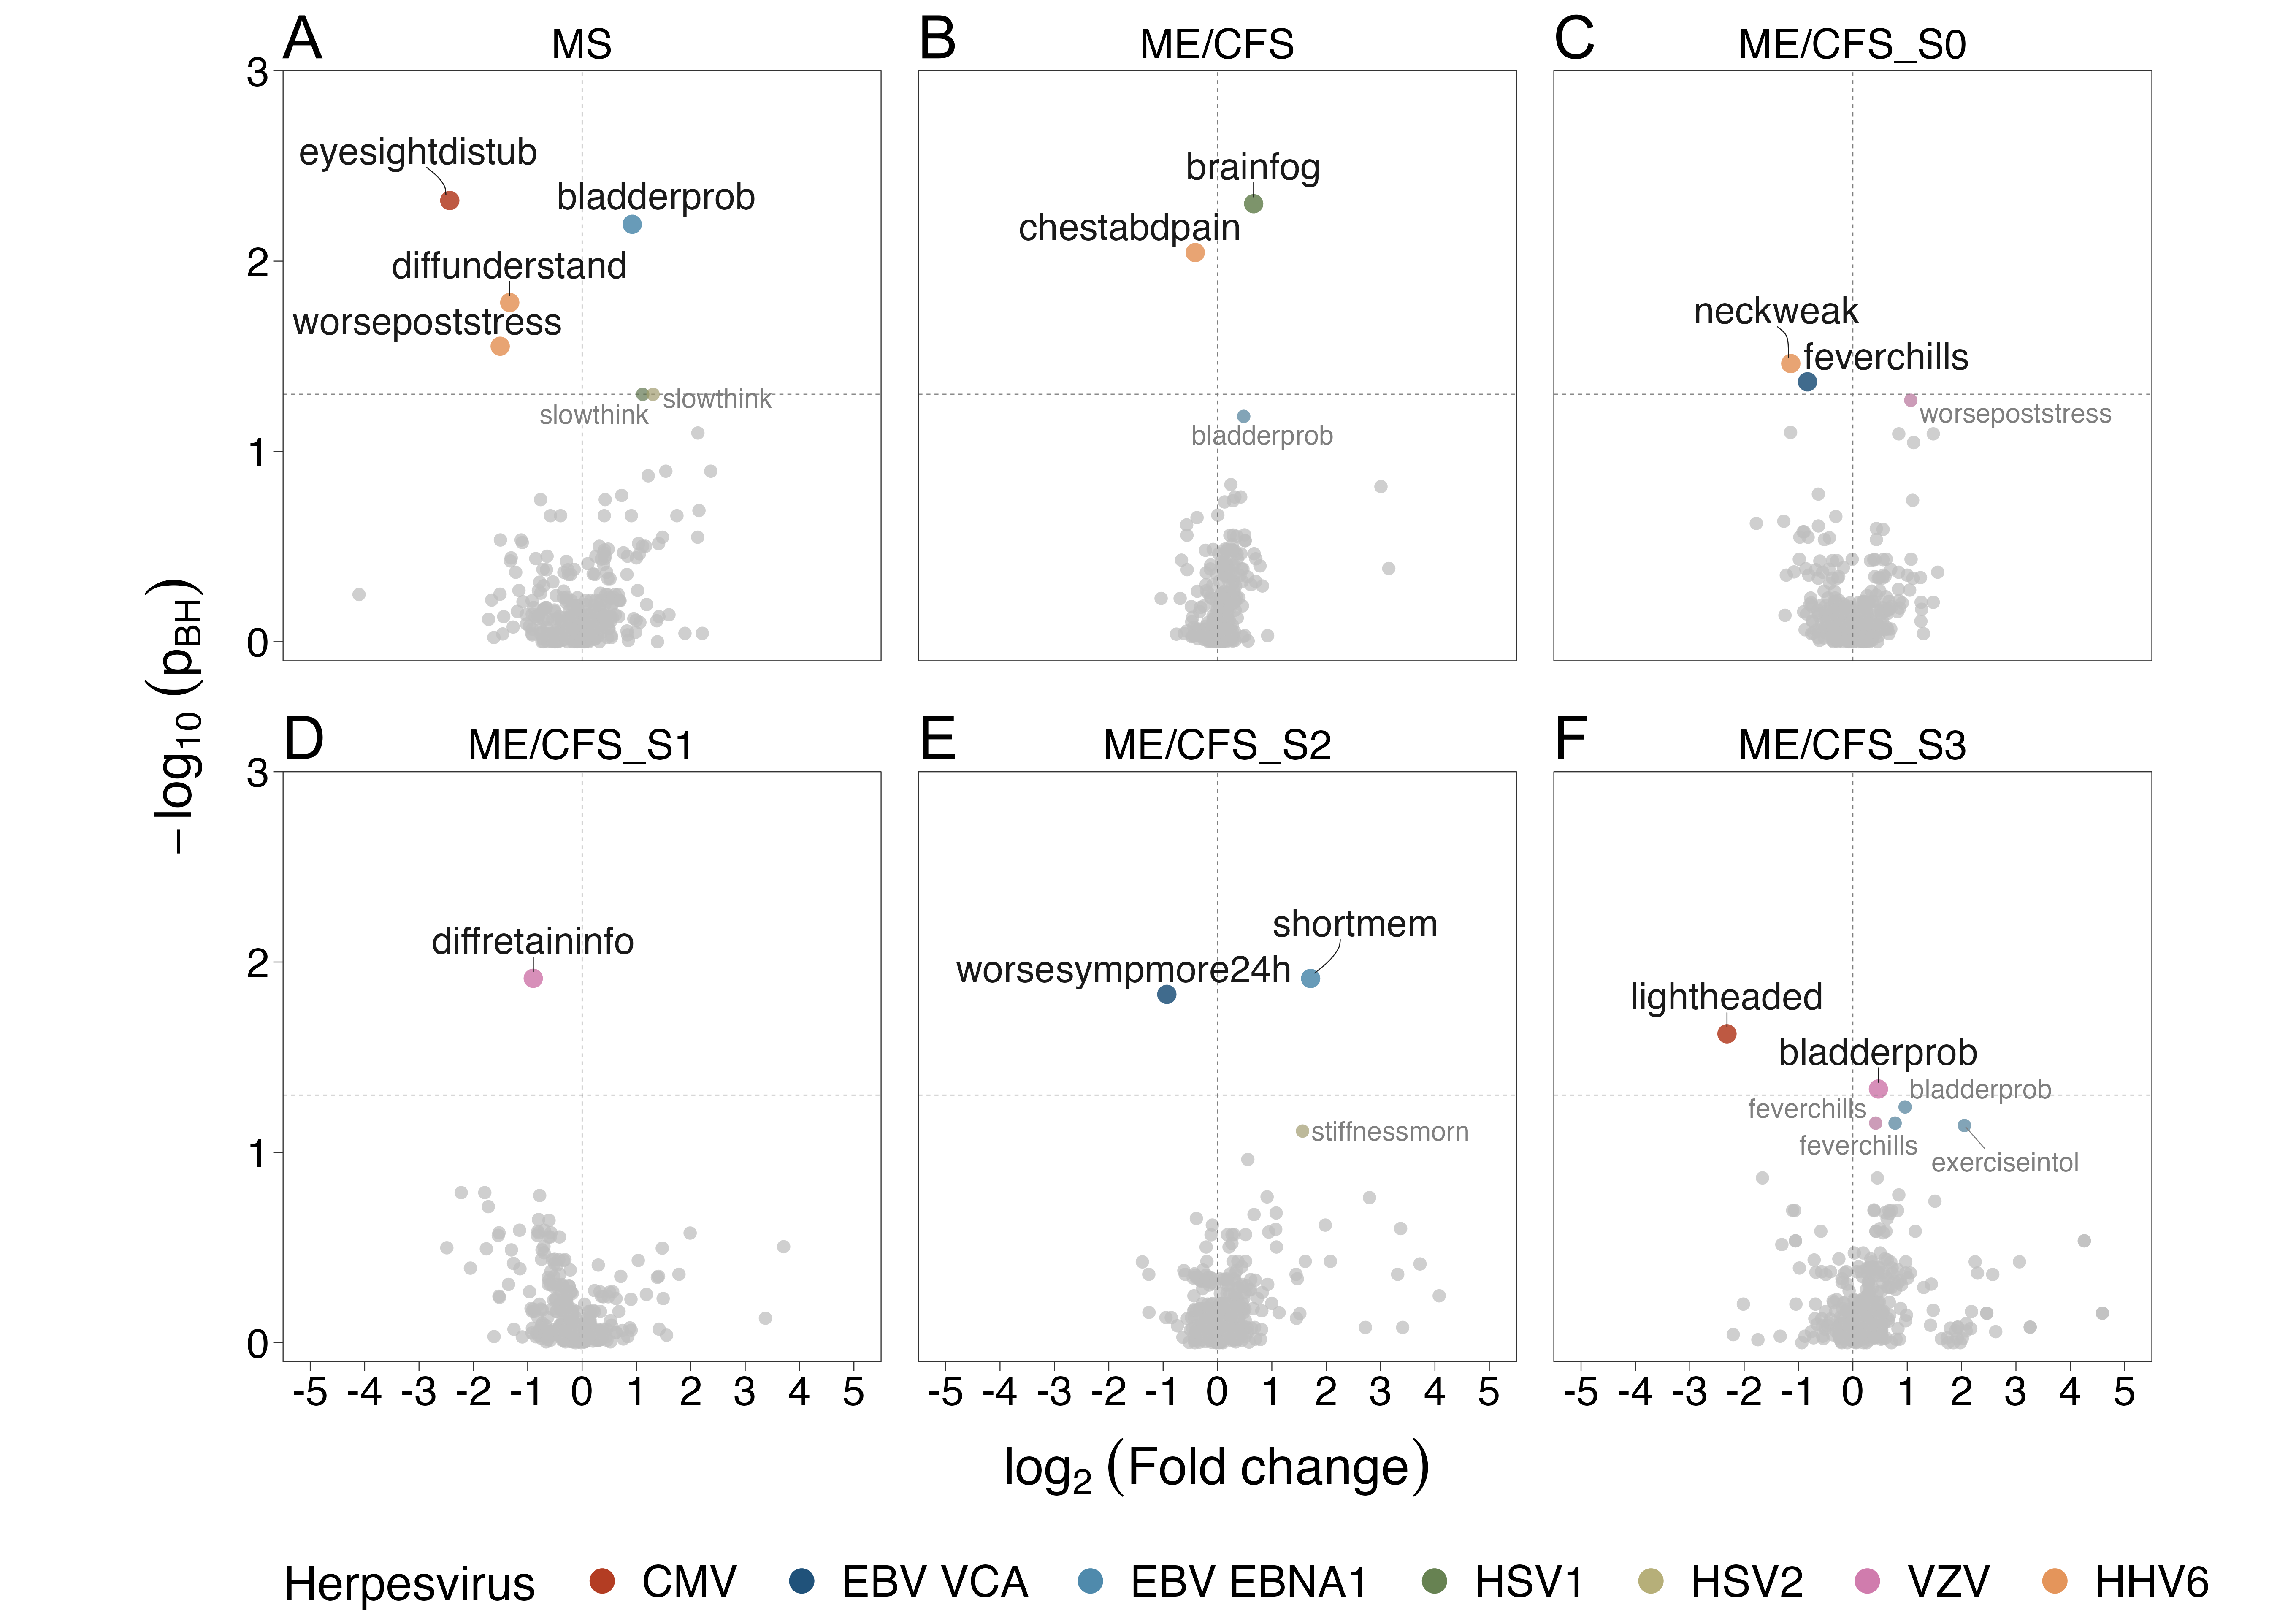
\includegraphics[width=0.95\textwidth]{chapter/2023-sym-and-herpesvirus/figures/fig5-association-anslysis-igg-and-cohorts.png}
    \caption[Association analysis between symptoms and IgG antibody data for the MS group and ME/CFS overall and stratified into subgroups]{Association analysis between symptoms and IgG antibody data for the MS group (A), the overall ME/CFS (B), the ME/CFS\_S0 subgroup (C), ME/CFS\_S1 subgroup (D), ME/CFS\_S2 subgroup (E), and ME/CFS\_S1 subgroup (F), where the $xx$ axis refers to $\log_{2}(\text{mean fold-change})$ between individuals with and without a given symptom, respectively, and the $yy$ axis refers to the logarithm in base 10 of the p-values derived from the Mann-Whitney test and adjusted for an FDR of 5\% using the Benjamini-Hochberg procedure ($-\log_{10}(\text{p}_\text{BH})$). See Supplementary Table~\ref{appendix:taba1-sym-bin-description} for linking the symptom codes presented in each plot to the respective symptom descriptions.}
    \label{fig:fig5-association-anslysis-igg-and-cohorts}
\end{figure}
% Figure 5
% Figure~\ref{fig:fig5-association-anslysis-igg-and-cohorts}

%%%%%%%%%%%%%%%%%%%%%%%%%%%%%%%%%%%%%%%%%%%%%%%%%%%%%%%%%%%%%%%%%%%%%%%%
%%%%%%%%%%%%%%%%%%%%%%%%%%%%%%%%%%%%%%%%%%%%%%%%%%%%%%%%%%%%%%%%%%%%%%%%
%%%%%%%%%%%%%%%%%%%%%%%%%%%%%%%%%%%%%%%%%%%%%%%%%%%%%%%%%%%%%%%%%%%%%%%%
\section{Discussion}

Our study showed that the overall ME/CFS cohort had more symptoms whose frequency was higher than the one observed for the MS patients. This finding was in agreement with a higher frequency of functional symptoms reported by an online self-report survey with the aim at finding the key differentiating symptoms of these two diseases \citep{jasonDifferentiatingMultipleSclerosis2017}. Interestingly, sore throat, tender glands, and flu-like symptoms from the immunological domain were also at the top differentiators of both ME/CFS\_S2 and ME/CFS\_S3 ME/CFS (i.e., subgroups related to a putative infectious trigger) and MS. Again, this finding is in line with another study where tender lymph nodes and flu-like symptoms could correctly distinguish MS from ME/CFS 81\% of the time \citep{ohanian2016IdentifyingKey}. Therefore, our study provided additional evidence that, besides the presence of hallmark persistent fatigue and PEM, symptoms from the immunological domain are crucial to diagnose ME/CFS and differentiate from MS. This is reflected in the CDC-1994 criterion and CCC-2003, two recommended case definitions for ME/CFS diagnosis, especially in the research setting \citep{nacul2021EuropeanNetwork}. However, we cannot rule out that difference in symptoms' frequency might be simply due to mild MS cases who did not undergo any treatment together with the presence of severely affected patients in the different ME/CFS subgroups. In this regard, it is important to emphasise that severe MS cases (most likely undergoing any immune-therapy) were excluded from participation in the UKMEB.

We found several positive and negative associations between herpesvirus antibody concentrations and different symptoms in each study group, even after adjusting for multiple testing. This finding is remarkable given the dozens of symptoms evaluated, the modest sample size of each study group, and the use of a non-parametric test that usually reduces the statistical power to detect group differences. However, we cannot rule out that these associations might be affected by patient's subjective perception of each symptom. At the same time, casting doubts on this perception is indirectly supporting theories that ME/CFS is a psychosomatic rather than an organic or a physical condition. A more plausible impact on the robustness of these associations is that they could have resulted from random fluctuations in symptomology occurring over the natural disease course. To confirm or refute this last explanation, one could conduct a longitudinal study with multiple timepoints and check whether the associations remain valid during follow-up.

The MS group had the highest number of significant antibody-symptom associations (or close to statistical significance). Therefore, infections by these herpesviruses seem to have a higher impact on this group than on the ME/CFS groups. The strongest association was observed for CMV antibody concentrations and the presence of eyesight disturbances. This is an interesting association given that photophobia and photosensitivity were commonly reported by MS patients \citep{cortese2018PhotophobiaMultiple} and CMV is also known to cause retinitis in immunocompromised individuals \citep{port2017CytomegalovirusRetinitis}. In this scenario, a reduction in antibodies against CMV might result in a low-grade ocular infection in MS patients. The second strongest association was found for EBNA1 antibody concentrations and bladder problems. This association is according to the view that bladder dysfunction, also a common symptom observed in MS, is linked to autoantibodies (for example, against muscarinic receptor-3) \citep{mccombe2009BladderDysfunction}. Our finding suggests that the origin of these autoantibodies could be a cross-reactive antibody response to an EBNA1 peptide mimicking a human protein, as demonstrated for MS \citep{ayoglu2016AnoctaminIdentified, tengvall2019MolecularMimicry, lanz2022ClonallyExpanded}. Interestingly, a positive association was also found for bladder problems in the ME/CFS\_S3 group but related to VZV antibody concentrations. Given that infections by VZV can also cause bladder dysfunction \citep{sakakibara2022VaricellazosterVirus}, we speculate that patients from this ME/CFS subgroup experienced a recent reactivation of the virus. Notwithstanding the recent observation of VZV reactivation after SARS-CoV-2 infections \citep{martinez-reviejo2022VaricellaZosterVirus} or under stressful conditions \citep{rooney2019HerpesVirus}, there is weak evidence for VZV reactivation in ME/CFS patients \citep{koelle2002MarkersViral, lee2021SalivaryDNA}. The remaining significant antibody-symptoms associations in the MS group were both negative and related to HHV6 IgG antibody concentrations. These associations are in opposition to the evidence that antibody concentrations to HHV6 are positively associated with the risk of developing MS \citep{engdahl2019IncreasedSerological}. A possible explanation for this contradicting finding is that a lower HHV6 antibody concentration triggers the reactivation of this virus, as observed in individuals after cord blood transplantation \citep{nakayama2021ImpactSpecific}. Unfortunately, the quantification of viral DNA was not performed in this study and, therefore, this explanation could not be tested with data.

As mentioned above, we found a lesser number of significant antibody-symptom associations in ME/CFS. Interestingly, the strongest association was found for increasing HSV1 antibody concentrations and brain fog. It is worth noting that brain fog is a colloquial term used by patients that seems to gather a constellation of symptoms mostly concerning deficits in cognition, such as reduced speed and efficiency of information processing, attention, concentration, and working memory \citep{ross2013WhatBrain, ocon2013CaughtThickness, krishnan2022MultidisciplinaryApproach}. If brain fog is taken in this sense, then the positive association with HSV1 antibody levels seems interesting given that this virus is known to be neurotropic during latency \citep{marcocci2020HerpesSimplex}. The presence and concentration levels of HSV1 IgG antibodies, as measured here, have been positively associated with cognitive deficits in both healthy individuals \citep{jonker2014AssociationExposure, tarter2014PersistentViral, fruchter2015ImpactHerpes} and patients suffering from Alzheimer's disease \citep{murphy2021HerpesSimplex}, schizophrenia \citep{dickerson2020AssociationExposure}, and bipolar disorder \citep{tucker2019AssessmentCognitive}. The same association could be significantly found for ME/CFS\_S1 and ME/CFS\_S2 before adjusting for multiple testing. Hence, a reduction in the statistical power by dividing patients in different strata is a plausible explanation for not finding this association in the ME/CFS subgroup analysis. At this point, it is reasonable to raise the question of why similar association with brain fog was not detected for antibody concentrations related to HHV6, another neurotropic virus whose viral miRNA was found in post-mortem brain biopsies of ME/CFS patients \citep{kasimir2022TissueSpecific}. A possible answer for this question is that, given that exposure to HHV6 is more prevalent in human populations than to HSV1, the respective antibody quantification has shorter dynamic range due to a high percentage of seropositive individuals (Table~\ref{tab:tab2-igg-antibodies.description} and Supplementary Figure~\ref{appendix:figa1-quantitative-serology}). In theory, this shorter dynamic range implies a higher sample size to detect smaller differences between patients reporting or not brain fog.

In the ME/CFS subgroup analysis, the detected antibody-symptom associations were not consistent across the 4 ME/CFS subgroups. This result suggested a large heterogeneity of different ME/CFS groups in terms of symptoms and their relationship with the underlying herpesviruses IgG antibody concentrations. An analysis based on disease severity could provide a clearer insight into the relationship between these two sets of variables. This possibility is motivated by a longitudinal study from the UKMEB where disease scores and different symptoms were associated with herpesvirus reactivation \citep{lee2021SalivaryDNA}. This alternative analysis by disease severity was beyond the scope of this study, but it will be done in a near future.

Our study also showed that the IgG antibody data were statistically significant to discriminate three ME/CFS subgroups from MS. Such a discrimination capability could be attributed to increased IgG antibody concentrations to multiple herpesviruses in the MS group, as previously found for EBV antigens \citep{loebel2017SerologicalProfiling}. This capability, although reaching statistical significance, is likely to have a diminished impact in the clinic, because it neither have a high sensitivity to classify these ME/CFS subgroups nor a high specificity to classify MS patients. This observation suggests that one should look for alternative disease-specific biomarkers or to combine these basic antibody measurements with more specific herpesvirus-related antibodies, such as those against EBNA4\_0529 and EBNA6\_0070 peptides derived from EBV \citep{sepulveda2022RevisitingIgG}. Notwithstanding this observation, it is worth mentioning that the reporting of a less promising finding helps the research community to focus on more promising biomarkers, thus, avoiding the waste of valuable research efforts and resources. It is also in line with the expectations of the UKMEB participants who are less concerned about breakthroughs in medical science and more interested in incremental steps and collaborative efforts which might one day lead to effective diagnosis, treatment, or cure \citep{lacerda2019HopeDisappointment}.

We found that serological data including the EBV antigens were unable to discriminate MS patients from the ME/CFS subgroup of patients who self-reported an infection (not evaluated by a lab test) at their disease onset. This subgroup is the largest in size and the one with the highest frequency of patients who self-reported a flu-like infection (22\%) or an unspecified viral infection (35\%) at their disease onset \citep{domingues2021HerpesvirusesSerologya}. Therefore, this subgroup seems very heterogeneous and non-specific. Given that many factors can contribute to MS pathogenesis \citep{marcocci2020HerpesSimplex}, the lack of evidence for a serological discrimination between these two groups might be attributed to the presence of multiple factors shared between this heterogeneous subgroup of ME/CFS patients and ME patients. In this line of thought, one could make the case for MS-related drugs such as cyclophosphamide \citep{patti2011LightsShadows} and rituximab \citep{brancati2021RituximabMultiple} to be deployed to treat ME/CFS patients, as made elsewhere \citep{flugeBLymphocyteDepletionPatients2019, rekeland2020IntravenousCyclophosphamide}. However, this deployment is likely to be more successful if targeting not all but only patients from this ME/CFS subgroup. However, future studies should be conducted to ascertain further similarities between this subgroup of ME/CFS patients and patients with MS.

There are four major limitations of this study. As already highlighted, the main limitation is that our re-analysis focused on data portraying a single snapshot of these patients. Given the fluctuating clinical course of ME/CFS (Table~\ref{tab:tab1-basic-characteristics-cfs-ms}), it is likely that the reported antibody-symptom associations might render irreproducible. It is also possible that non-significant associations would become statistically (and clinically) significant in latter time points. A longitudinal study including the measurements at multiple time points would resolve this limitation. In practice, such a study is expensive and affected by other problems, such as patients' compliance or the presence of missing data due to drop-outs. Patient's exhaustion (often triggered by data collection) is also another limiting factor in the context of ME/CFS research. As such, the common and pragmatic approach is to conduct association analyses between different biomarkers and symptoms (or, alternatively, symptom scores) using cross-sectional data, as illustrated not only for ME/CFS but also for Long Covid \citep{freitag2021AutoantibodiesVasoregulative, blauensteiner2021AlteredEndothelial, szklarski2021DelineatingAssociationa, sotzny2022DysregulatedAutoantibodies}.

The second limitation is that IgG antibodies are often used as biomarkers of a past active infection. As such, these antibodies have limited power to judge when the last active infection occurred and whether these herpesviruses are currently active or simply latent. In this regard, our study would have benefited from a quantification of IgM antibodies in the same biological samples. However, additional serological testing was beyond the scope of this study due to lack of funding and inexistence of biological material for many of the study participants. In this scenario, our study should be viewed as an opportunistic re-analysis of already existing data with its own limitations.

The third limitation is that the MS cohort was conveniently enrolled in the UKMEB due to the criterion of excluding any patient following any immune therapy. In this perspective, the recruited MS patients can be seen as ``pure patients'' or simply ``mild cases''. On the one hand, the recruitment of patients without any treatment suggests a selective bias towards sampling patients with less severe symptoms, thus, explaining the higher number of symptoms that are more prevalent in the ME/CFS group than in the MS one. This putative bias was also suggested by a higher number of symptoms whose frequency was similar in MS and ME/CFS\_S0/ME/CFS\_S1 in which the frequency of severely affected patients was less than 10\%. However, low adherence to modifying disease therapy by MS patients is considered a major concern in the management of the disease \citep{cerghet2010AdherenceDiseaseModifying, rieckmann2015AchievingPatient} and, therefore, the recruited MS patients are in part representative of this clinical population who do not adhere to any treatment.

The fourth limitation is that disease course profiles do not comply with the standard classification used in MS research; this standard classification is reviewed elsewhere \citep{klineova2018ClinicalCourse}. These profiles, if following such a standard, would have helped to understand whether the proportions of sampled MS patients at different disease courses would match those found across epidemiological studies of MS, thus, increasing the interpretation on the representativeness of the MS cohort. Notwithstanding this limitation, 22\% of the MS patients reported constantly getting worse. This frequency anecdotally coincides with the prevalence of a primary progressive disease course (15\%--22\%) in MS patients from different parts of the UK \citep{pugliatti2006EpidemiologyMultiple}. In addition, all study groups were well matched for the alternative disease course categorisation used here and, therefore, there is evidence that our findings are less likely to be driven by differences in putative disease courses of the patients.

In conclusion, some candidate antibody-symptom associations were identified for ME/CFS patients. However, the clinical impact of these associations remains to be determined given the fluctuating nature of symptoms in ME/CFS patients and the nature of IgG antibodies in simply detecting exposure. To understand the true impact of our findings in the clinic, we propose a future longitudinal study with at least three timepoints. This study is likely to help discerning the robustness of the reported associations during disease course and whether they could be targeted by any existing drug treatment. This study, although theoretical appealing, might be difficult to design with an appropriate statistical power and to execute in the clinic given the lack of funding affecting ME/CFS research, poor societal recognition of the disease, and possible patient's exhaustion during follow-up.
% \vfill
% \newpage

%%%%%%%%%%%%%%%%%%%%%%%%%%%%%%%%%%%%%%%%%%%%%%%%%%%%%%%%%%%%%%%%%%%%%%%%
\addcontentsline{toc}{section}{Bibliography}
\bibliographystyle{abbrvnat}
\bibliography{references}
%%%%%%%%%%%%%%%%%%%%%%%%%%%%%%%%%%%%%%%%%%%%%%%%%%%%%%%%%%%%%%%%%%%%%%%%


% Table 1
% Table~\ref{tab:tab1-basic-characteristics-cfs-ms}
% Table 2
% Table~\ref{tab:tab2-igg-antibodies.description}
% Table 3
% Table~\ref{tab:tab3-models-auc-optimal-cutoff-se-sp}

% Figure 1
% Figure~\ref{fig:fig1-age-adj-or-cfs-all-vs-ms}
% Figure 2
% Figure~\ref{fig:fig2-age-adj-or-cfs-other-vs-ms}
% Figure 3
% Figure~\ref{fig:fig3-roc-curves-sl-algorithm}
% Figure 4
% Figure~\ref{fig:fig4-smooth-line-approximations}
% Figure 5
% Figure~\ref{fig:fig5-association-anslysis-igg-and-cohorts}

% Supplementary Table 1
% Supplementary Table~\ref{appendix:taba1-sym-bin-description}
% Supplementary Table 2
% Supplementary Table~\ref{appendix:taba2-percentage-sym-bin}
% Supplementary Table 3
% Supplementary Table~\ref{appendix:taba3-models-auc-optimal-cutoff-ms}

% Supplementary Figure 1
% Supplementary Figure~\ref{appendix:figa1-quantitative-serology}
% Supplementary Figure 2

% Supplementary Figure 3

% Supplementary Figure  4
